\documentclass[12pt, a4paper]{article}

% ── Packages ─────────────────────────────────────────────────────────────────
\usepackage[a4paper, margin=2.5cm]{geometry}
\usepackage{amsmath, amssymb, amsthm}
\usepackage{graphicx}
\usepackage{booktabs}
\usepackage{array}
\usepackage{listings}
\usepackage{xcolor}
\usepackage{hyperref}
\usepackage{natbib}
\usepackage{setspace}
\usepackage{titlesec}
\usepackage{abstract}
\usepackage{microtype}
\usepackage{parskip}
\usepackage[ruled, vlined, linesnumbered]{algorithm2e}
\usepackage{mdframed}
\usepackage{tikz}
\usetikzlibrary{arrows.meta, positioning, calc}
\usepackage{adjustbox}
\usepackage{float}
\graphicspath{{outputs/figures/}}

% ── Hyperref setup ────────────────────────────────────────────────────────────
\hypersetup{
  colorlinks = true,
  linkcolor  = blue!60!black,
  citecolor  = blue!60!black,
  urlcolor   = blue!60!black,
  pdftitle   = {A Hierarchical Vector-Based Framework for Multi-Scale Exploded-View Cartography},
  pdfauthor  = {}
}

% ── Section title formatting ─────────────────────────────────────────────────
\titleformat{\section}{\large\bfseries}{\thesection.}{0.6em}{}
\titleformat{\subsection}{\normalsize\bfseries}{\thesubsection}{0.6em}{}
\titleformat{\subsubsection}{\normalsize\itshape}{\thesubsubsection}{0.6em}{}

% ── Code listing style ────────────────────────────────────────────────────────
\lstdefinestyle{Rstyle}{
  language        = R,
  basicstyle      = \ttfamily\small,
  keywordstyle    = \color{blue!70!black}\bfseries,
  commentstyle    = \color{gray},
  stringstyle     = \color{orange!80!black},
  numbers         = left,
  numberstyle     = \tiny\color{gray},
  numbersep       = 8pt,
  breaklines      = true,
  frame           = single,
  framerule       = 0.4pt,
  rulecolor       = \color{gray!40},
  backgroundcolor = \color{gray!5},
  captionpos      = b,
  showstringspaces= false,
  tabsize         = 2
}
\lstset{style=Rstyle}

% ── Theorem-like environments ─────────────────────────────────────────────────
\newmdtheoremenv[
  linecolor  = blue!50!black,
  linewidth  = 1pt,
  topline    = true,
  bottomline = true,
  rightline  = false,
  leftline   = false,
  innertopmargin  = 6pt,
  innerbottommargin = 6pt
]{definition}{Definition}

% ── Equation numbering ────────────────────────────────────────────────────────
\numberwithin{equation}{section}

% ── Spacing ───────────────────────────────────────────────────────────────────
\setlength{\parskip}{6pt}
\onehalfspacing

% ─────────────────────────────────────────────────────────────────────────────
\begin{document}

% ── Title ─────────────────────────────────────────────────────────────────────
\begin{titlepage}
  \centering
  \vspace*{2cm}
  {\LARGE\bfseries A Hierarchical Vector-Based Framework for\\[4pt]
   Multi-Scale Exploded-View Cartography\par}
  \vspace{0.8cm}
  {\large\itshape Centroid-Driven Spatial Displacement for Dense Administrative Maps\par}
  \vspace{1.2cm}
  {\large George Arthur\par}
  \vspace{1cm}
  {\small
  \textbf{Keywords:} exploded-view maps; cartographic generalization; spatial displacement;\\
  vector-field deformation; hierarchical cartography; administrative boundaries;\\
  geovisualization; computational cartography\par}
  \vfill
\end{titlepage}

% ── Abstract ──────────────────────────────────────────────────────────────────
\begin{abstract}
\noindent
Exploded-view cartography provides a method for improving the readability of dense administrative maps by introducing controlled spatial separation between geographic units while preserving their internal geometry. Despite its practical value, exploded layouts are typically produced through manual tuning or heuristic displacement rules, limiting reproducibility and portability across datasets.

This paper introduces a hierarchical vector-based framework for generating exploded administrative maps using centroid-driven displacement fields. The method translates polygon geometries using a deterministic vector formulation derived from hierarchical centroid relationships, allowing simultaneous separation at multiple administrative levels while preserving the internal morphology of each geographic unit exactly through rigid-body translation.

We derive functional forms for the two principal displacement parameters governing regional separation and intra-region expansion. The regional parameter is derived from a radial gap model describing the chord-length increase when parent regions are displaced outward from a shared centroid. The local parameter is derived from an equal-area partition model approximating the characteristic spacing of municipal units within a region. These derivations determine the structural dependence of the parameters on geometric quantities---characteristic polygon diameter, regional radius, and municipal density---leaving only dimensionless clearance coefficients to be calibrated empirically. This formulation substantially reduces manual parameter tuning while retaining interpretable legibility coefficients.

The framework is evaluated using municipal boundary data from New Jersey ($n = 564$ municipalities, 3 regions) and applied to Pennsylvania ($n = 2{,}572$ municipalities, 6 regions) as a large-scale transfer test. Additional reproducible cases cover Ohio, Michigan, Kentucky, Illinois, North Dakota, North Carolina, Virginia, Texas, Florida, Canada, Germany, and a 10-region U.S.\ HHS grouped layout. The NJ-calibrated local coefficient $\gamma_l$ provides a useful transferable starting value, but the evidence is presented as preliminary validation rather than proof of a universal constant. For publication-quality figures, a documented rigid display-offset layer is applied after formula-derived displacement and recorded as CSV input.

Because the closed-form displacement step operates through direct vector translation without iterative optimization or topology reconstruction, it is $O(n)$ in feature count, excluding geometry preprocessing, CRS transformation, union/centroid operations, and optional refinement. The method is therefore suitable for dynamic mapping environments such as interactive web applications and statistical dashboards. The accompanying \textsf{R} implementation and map gallery provide reproducible scripts, static outputs, and documented display offsets separating analytical validation from cartographic finishing.
\end{abstract}

\newpage
\tableofcontents
\newpage

% ─────────────────────────────────────────────────────────────────────────────
\section{Introduction}
% ─────────────────────────────────────────────────────────────────────────────

Thematic maps of administrative regions become difficult to read when rendered in a conventional geographic layout. Dense municipal, county, or district boundaries create visual congestion, making it hard to distinguish adjacent units, perceive higher-level structure, or support interactive tasks such as hovering, clicking, or labeling. These challenges are especially pronounced in the northeastern United States and other regions characterized by fine-grained political subdivision. New Jersey, with over 560 municipalities distributed across a compact geographic area, is a representative example.

Cartography has long addressed such problems through generalization operations including simplification, aggregation, typification, and displacement. Among these, displacement is particularly important when geographic objects must be moved to improve readability while retaining spatial relationships. However, many existing displacement methods are formulated as optimization problems or iterative conflict-resolution procedures, which are computationally demanding and difficult to deploy in dynamic web-based environments \citep{bader2001, harrie2002}.

An alternative strategy is to create an \emph{exploded-view} cartographic layout, in which spatial units are separated to introduce whitespace while preserving their original geometry. Although exploded layouts are familiar in engineering illustration and some forms of schematic cartography, they remain relatively under-formalized for hierarchical administrative maps. There is limited prior work on deterministic, geometry-preserving exploded layouts that support both hierarchical separation and computational efficiency.

This paper proposes a hierarchical centroid-driven displacement framework for exploded-view cartography. The method treats displacement as a vector field over the map domain and computes translations analytically from centroid relationships across administrative levels. Rather than iteratively resolving collisions, it defines displacement directly from parent-child spatial structure. The result is a closed-form, multi-scale, geometry-preserving transformation that connects naturally to established traditions in cartogram deformation, flow map visualization, and cartographic distortion analysis.

\paragraph{Contributions.} The main contributions of this work are:
\begin{enumerate}
  \item We formalize a hierarchical piecewise-rigid displacement approach for exploded-view administrative cartography, in which each feature undergoes rigid-body motion while displacement vectors are sampled from centroid-derived radial potentials. This places the method between rigid transforms, continuous deformation, and topological rearrangements.
  \item A rigid-body translation framework (Proposition~1) guaranteeing exact preservation of feature shape, area, perimeter, and topological structure --- unlike cartogram and deformation methods that warp geometry.
  \item Geometry-derived parameter formulas (Analytical Results~1--2) linking displacement magnitude to intrinsic dataset properties, constituting a reusable parameterization procedure applicable to any administrative polygon dataset with a defined hierarchy.
  \item A closed-form displacement step that is $O(n)$ in feature count, with a zoom-dependent extension $t_i(z) = \lambda(z)\cdot t_i$ for interactive multi-scale layouts.
  \item A three-level multi-scale extension enabling grouped national layouts through automatic anchor generation and collision-aware anchor refinement with spring stabilization (Section~\ref{sec:multiscale}).
  \item A generalized open \textsf{R} package implementation exposing \texttt{explode\_sf()}, \texttt{explode\_state()}, \texttt{explode\_sf\_with\_lookup()}, and \texttt{apply\_region\_offsets()} for administrative polygon datasets without modification to the core algorithm (Section~\ref{sec:genimpl}), together with a companion focus-map widget for interactive selected-feature inspection.
\end{enumerate}

% ─────────────────────────────────────────────────────────────────────────────
\section{Related Work}
% ─────────────────────────────────────────────────────────────────────────────

The proposed method sits at the intersection of four cartographic research traditions.

\subsection{Cartographic Generalization and Displacement}

Cartographic generalization provides the conceptual foundation for this work. Displacement is one of its core operators, used when map objects must be moved to avoid overlap or improve readability while preserving relevant spatial relations \citep{wu2021, mackaness2011}. A major strand of displacement research formulates the problem as optimization or energy minimization. \citet{bader2001} treats feature displacement as an energy minimization problem, and \citet{harrie2002} describe simultaneous graphic generalization of vector datasets under competing cartographic constraints. These methods are powerful but computationally expensive, limiting their use in real-time or interactive mapping.

\subsection{Vector-Field Models and Map Deformation}

A second relevant strand represents displacement as a spatially varying deformation field. \citet{ai2015} propose a vector-field model for handling multiple displacement conflicts in building generalization, showing how conflict resolution can be expressed through displacement fields rather than object-by-object adjustment. Related work on distortion analysis uses vector fields to visualize how maps differ from reference geometries \citep{jenny2011}.

The method developed here belongs to this family: displacement is expressed as a closed-form hierarchical vector field whose components are defined by parent-child centroid relationships rather than by iterative force propagation.

\subsection{Cartograms and Spatial Transformation}

Cartograms transform geographic space by defining a displacement field over the map domain. In diffusion-based cartograms, the map is warped according to a field induced by density equalization \citep{gastner2004}. Force-based approaches generate similar transformations through spring relaxation \citep{sun2020}. Reviews of cartogram methods emphasize the trade-off between distortion, topology, orientation, and recognizability \citep{nusrat2016}.

The present method differs from cartograms in a crucial respect: it does not deform polygon interiors. Each administrative unit undergoes rigid-body translation, preserving shape and area exactly. Nevertheless, the displacement field shares the mathematical structure $T(x) = x + V(x)$ common to cartogram transformations.

\subsection{Hierarchy and Multi-Scale Cartography}

Hierarchical data structures are central to multi-scale mapping. \citet{cecconi2003} highlights the need for hierarchical representations supporting changing scale and display conditions. More recent discussions emphasize that hierarchy is fundamental to organizing cartographic operations across scales \citep{bundy2020, yan2019}. The framework proposed here builds directly on this principle: hierarchy is not merely an organizational device but the source of the displacement field itself.

\subsection{Position of the Present Work}

The method differs from prior work in three main respects. First, it produces an exploded-view layout rather than a conflict-only displacement. Second, it is deterministic and closed-form, avoiding iterative optimization. Third, it defines displacement from hierarchical centroid structure, yielding a lightweight multi-scale method suited to real-time visualization.

More broadly, existing cartographic transformations include rigid transforms (translation, rotation, scaling), continuous deformation (cartograms, rubber-sheet maps, diffusion-based warping), and topological rearrangements (schematic maps, grid maps). The present method formalizes a \emph{piecewise rigid hierarchical displacement} approach: each feature undergoes rigid-body motion, while the displacement vectors are sampled from centroid-derived radial potentials. To our knowledge, this specific combination has not been systematically formalized for administrative exploded-view cartography.

% ─────────────────────────────────────────────────────────────────────────────
\section{Methodology}
% ─────────────────────────────────────────────────────────────────────────────

\subsection{Formal Problem Statement}

The algorithm is packaged as a reusable function:
\[
  \texttt{explode\_map}(G,\ \text{hierarchy},\ \alpha_r,\ \alpha_l,\ p)
\]
with inputs:
\begin{itemize}
  \item $G = \{G_i\}$ --- a set of vector polygon geometries (administrative units),
  \item $\text{hierarchy}$ --- a two-level assignment mapping each unit $i$ to a parent region $r(i)$ and a global frame $s$ (e.g., state),
  \item $\alpha_r \in \mathbb{R}_{>0}$ --- global displacement scale,
  \item $\alpha_l \in \mathbb{R}_{>0}$ --- local displacement scale,
  \item $p > 0$ --- distance scaling exponent,
\end{itemize}
and output $G' = \{G'_i\}$, a set of exploded vector geometries identical in shape and area to $G$.

\subsection{Rigid-Body Translation Model}

Let $G_i$ denote the geometry of administrative unit $i$. The exploded geometry is produced by a rigid-body translation:
\begin{equation}
  G'_i = G_i + t_i
  \label{eq:translation}
\end{equation}
where $t_i \in \mathbb{R}^2$ is a constant displacement vector applied uniformly to every point of $G_i$. The problem therefore reduces to computing a $t_i$ that introduces legible whitespace while maintaining recognizable spatial structure.

\begin{mdframed}[linecolor=blue!50!black, linewidth=1pt, topline=true, bottomline=true, rightline=false, leftline=false, innertopmargin=6pt, innerbottommargin=6pt]
\textbf{Proposition 1} (Feature-level geometry preservation). \textit{Let $G_i \subset \mathbb{R}^2$ be a valid polygonal administrative unit and let $G'_i = G_i + t_i$ for a constant vector $t_i \in \mathbb{R}^2$. Then $T_i(x) = x + t_i$ preserves the internal geometry of $G_i$, including shape, area, perimeter, orientation, and topological structure.}

\smallskip
\textit{Proof.} For any $x, y \in G_i$,
\[
  \|T_i(x) - T_i(y)\| = \|(x + t_i) - (y + t_i)\| = \|x - y\|
\]
so all pairwise distances within $G_i$ are preserved. Since translation is an isometry of $\mathbb{R}^2$, it preserves angle relationships, orientation, boundary structure, and area (Jacobian determinant = 1). Therefore $G'_i$ is congruent to $G_i$ and its internal topology is unchanged. $\square$
\end{mdframed}

\smallskip
\noindent\textbf{Scope of preservation.} Proposition~1 applies within each individual polygon. Across distinct units, adjacency relations and shared-boundary coincidence are \emph{not} automatically preserved after displacement; see Section~\ref{sec:discussion} for a precise statement of this limitation.

\subsection{Centroid Definitions}

Three centroid levels are defined:
\begin{align}
  C_i        &= \text{centroid}(G_i) & &\text{(unit centroid)} \label{eq:ci}\\
  C_{r(i)}   &= \text{centroid}\!\left(\bigcup_{j \in r(i)} G_j\right) & &\text{(region centroid)} \label{eq:cr}\\
  C_s        &= \text{centroid}\!\left(\bigcup_i G_i\right) & &\text{(state centroid)} \label{eq:cs}
\end{align}

\begin{figure}[H]
\centering
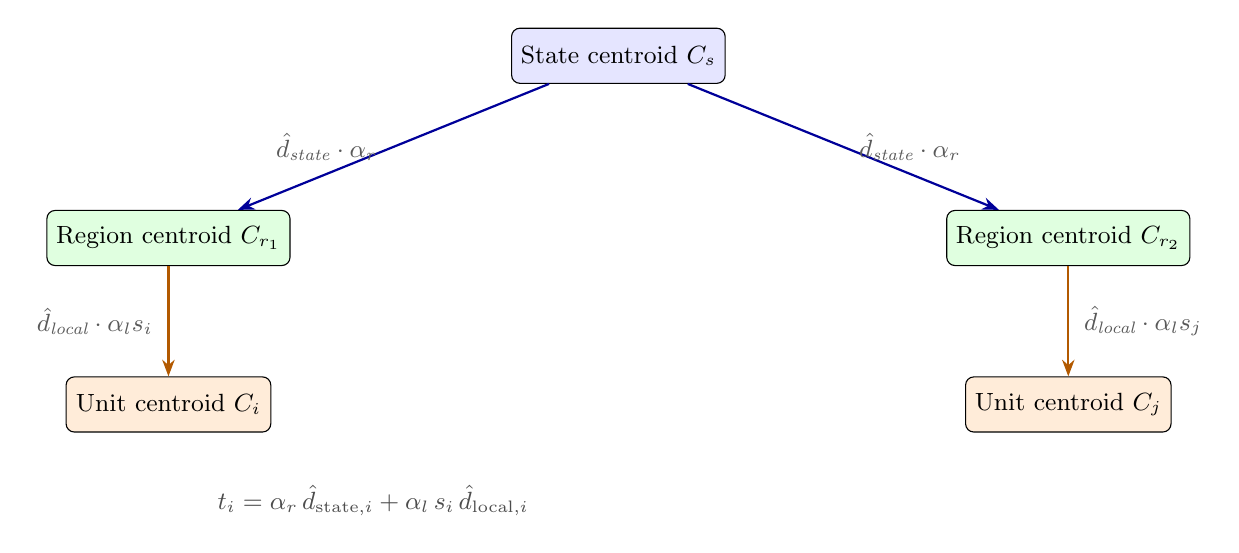
\begin{tikzpicture}[
  node distance  = 1.6cm and 2.8cm,
  box/.style     = {draw, rounded corners=3pt, minimum width=2.6cm,
                    minimum height=0.7cm, align=center, font=\small},
  arrow/.style   = {-{Stealth[length=6pt]}, thick},
  label/.style   = {font=\small\itshape, text=gray!70!black}
]

% ── Nodes ────────────────────────────────────────────────────────────────────
\node[box, fill=blue!10]  (cs)  {State centroid $C_s$};
\node[box, fill=green!12, below left=of cs]  (cr1) {Region centroid $C_{r_1}$};
\node[box, fill=green!12, below right=of cs] (cr2) {Region centroid $C_{r_2}$};
\node[box, fill=orange!15, below=1.4cm of cr1] (ci1) {Unit centroid $C_i$};
\node[box, fill=orange!15, below=1.4cm of cr2] (ci2) {Unit centroid $C_j$};

% ── Regional arrows ──────────────────────────────────────────────────────────
\draw[arrow, blue!60!black]
  (cs) -- node[label, left=2pt]  {$\hat{d}_{\text{state}} \cdot \alpha_r$} (cr1);
\draw[arrow, blue!60!black]
  (cs) -- node[label, right=2pt] {$\hat{d}_{\text{state}} \cdot \alpha_r$} (cr2);

% ── Local arrows ─────────────────────────────────────────────────────────────
\draw[arrow, orange!70!black]
  (cr1) -- node[label, left=2pt]  {$\hat{d}_{\text{local}} \cdot \alpha_l s_i$} (ci1);
\draw[arrow, orange!70!black]
  (cr2) -- node[label, right=2pt] {$\hat{d}_{\text{local}} \cdot \alpha_l s_j$} (ci2);

% ── Total displacement annotation ────────────────────────────────────────────
\node[font=\small, align=center, text=gray!60!black,
      below=0.55cm of ci1, xshift=2.6cm]
  {$t_i = \alpha_r\,\hat{d}_{\text{state},i} + \alpha_l\,s_i\,\hat{d}_{\text{local},i}$};

\end{tikzpicture}
\caption{Hierarchical displacement model. Each administrative unit $i$ receives
a total translation $t_i$ composed of two centroid-derived vectors: a
\textcolor{blue!60!black}{regional component} (blue) displacing the parent region away from the
state centroid, and a \textcolor{orange!70!black}{local component} (orange) displacing the unit
away from its region centroid, scaled by $s_i$ to suppress voids near regional centroids.}
\label{fig:hierarchy}
\end{figure}

\subsection{Direction Vectors}

Two normalized direction vectors are derived from these centroids.

The \emph{regional direction vector} points from the state centroid toward the parent region centroid:
\begin{equation}
  \hat{d}_{\text{state},i} = \frac{C_{r(i)} - C_s}{\|C_{r(i)} - C_s\|}
  \label{eq:dstate}
\end{equation}

The \emph{local direction vector} points from the region centroid toward the unit centroid:
\begin{equation}
  \hat{d}_{\text{local},i} = \frac{C_i - C_{r(i)}}{\|C_i - C_{r(i)}\|}
  \label{eq:dlocal}
\end{equation}

\noindent\textbf{Degenerate cases.} The implementation uses deterministic zero-vector fallbacks for singular configurations. If $\|C_{r(i)} - C_s\| = 0$, the regional direction is set to $(0,0)$ for that parent region. If $\|C_i - C_{r(i)}\| = 0$, the local direction is set to $(0,0)$ for that unit. If a parent region contains only one child unit or $d_{\max,r}=0$, then $s_i=0$ for all units in that region. Empty geometries fail validation; invalid geometries should be repaired before displacement or rejected with an explicit error. For multipart polygons, centroids are area-weighted centroids of the geometry in the working projected CRS; point-on-surface locations are used only for label placement, not for displacement vectors.

\subsection{Distance-Scaled Local Expansion}

A naïve local displacement model assigns approximately equal magnitude to all units after normalization, tending to create excessive hollow regions near parent centroids. To control this effect, the local term is modulated by a normalized distance scaling coefficient:
\begin{equation}
  s_i = \left(\frac{\|C_i - C_{r(i)}\|}{d_{\max,r(i)}}\right)^{p}
  \label{eq:si}
\end{equation}
where
\begin{equation}
  d_{\max,r(i)} = \max_{j \in r(i)} \|C_j - C_{r(i)}\|
  \label{eq:dmax}
\end{equation}
is the maximum unit-to-region-centroid distance within region $r(i)$, and $p \geq 1$ controls non-linearity. For $p > 1$, units near the regional centroid receive disproportionately reduced displacement, further suppressing void formation.

A key consequence of this design is that the local expansion is a monotonic function of radial distance from the region centroid.

\begin{mdframed}[linecolor=blue!50!black, linewidth=1pt, topline=true, bottomline=true, rightline=false, leftline=false, innertopmargin=6pt, innerbottommargin=6pt]
\textbf{Proposition 2} (Radial ordering preservation). \textit{Let units $i$ and $j$ belong to the same region $r$, and let their centroids satisfy $\|C_i - C_r\| < \|C_j - C_r\|$. Then after displacement, $\|C'_i - C'_r\| < \|C'_j - C'_r\|$, where $C'_r = C_r + \alpha_r\,\hat{d}_{\textup{state},r}$ is the displaced region centroid. That is, radial ordering of units within a region is preserved by the transformation.}

\smallskip
\textit{Proof.} Let $r_i = \|C_i - C_r\|$ and $r_j = \|C_j - C_r\|$ with $r_i < r_j$. The local displacement of each unit along its radial direction is:
\[
  \delta_i = \alpha_l\, s_i = \alpha_l \left(\frac{r_i}{d_{\max}}\right)^p, \qquad
  \delta_j = \alpha_l\, s_j = \alpha_l \left(\frac{r_j}{d_{\max}}\right)^p
\]
Since $r_i < r_j$ and $p > 0$, we have $\delta_i < \delta_j$. Each unit is displaced along its own unit vector $\hat{d}_{\text{local}}$ away from $C_r$, so the displaced radial distance satisfies:
\[
  \|C'_i - C'_r\| = r_i + \delta_i, \qquad \|C'_j - C'_r\| = r_j + \delta_j
\]
(both centroids move by the same $\alpha_r\,\hat{d}_{\text{state},r}$ term, which cancels in the difference). Since $r_i < r_j$ and $\delta_i < \delta_j$, it follows immediately that $r_i + \delta_i < r_j + \delta_j$. $\square$
\end{mdframed}

\smallskip
\noindent\textbf{Interpretation.} Proposition~2 guarantees that units closer to their regional centroid in geographic space remain closer after displacement --- the transformation expands the region outward like a radial elastic sheet rather than shuffling units in the radial direction. This property contributes directly to the perceptual stability of the exploded layout: the human visual system reads the result as coherent radial expansion rather than random repositioning. It also explains why dense urban cores (e.g., the Philadelphia and Pittsburgh metropolitan clusters in the Pennsylvania case study) remain correctly suppressed near their regional centroids rather than being pushed outward past sparser surrounding municipalities.

\subsection{Total Displacement Vector}

The final displacement vector combines both components:
\begin{equation}
  \boxed{t_i = \alpha_r\,\hat{d}_{\text{state},i} + \alpha_l\,s_i\,\hat{d}_{\text{local},i}}
  \label{eq:ti}
\end{equation}
where $\alpha_r$ controls separation among parent regions and $\alpha_l$ controls local expansion within each region. The transformed geometry follows directly from~\eqref{eq:translation}.

\begin{mdframed}[linecolor=blue!50!black, linewidth=1pt, topline=true, bottomline=true, rightline=false, leftline=false, innertopmargin=6pt, innerbottommargin=6pt]
\textbf{Proposition 3} (Bounded displacement). \textit{Let $t_i$ be defined as in Equation~\eqref{eq:ti}. Then:}
\[
  \|t_i\| \leq \alpha_r + \alpha_l
\]
\textit{That is, no feature can be displaced by more than $\alpha_r + \alpha_l$ from its original position.}

\smallskip
\textit{Proof.} Since $\hat{d}_{\text{state},i}$ and $\hat{d}_{\text{local},i}$ are unit vectors and $0 \leq s_i \leq 1$, the triangle inequality gives:
\[
  \|t_i\| = \|\alpha_r\,\hat{d}_{\text{state},i} + \alpha_l\,s_i\,\hat{d}_{\text{local},i}\|
           \leq \alpha_r\|\hat{d}_{\text{state},i}\| + \alpha_l\,s_i\|\hat{d}_{\text{local},i}\|
           = \alpha_r + \alpha_l\,s_i \leq \alpha_r + \alpha_l \quad \square
\]
\end{mdframed}

\smallskip
\noindent\textbf{Interpretation.} Proposition~3 provides a global stability guarantee: the displacement magnitude of every feature is predictable and controlled entirely by the two scale parameters. The layout cannot diverge regardless of the number of units or the complexity of the hierarchy. This property distinguishes the method from iterative force-based displacement algorithms, which may exhibit runaway displacement under certain configurations. The bound is tight: it is achieved when $s_i = 1$ (a unit at the maximum distance from its regional centroid) and when $\hat{d}_{\text{state},i}$ and $\hat{d}_{\text{local},i}$ are parallel.

The framework does not guarantee global non-overlap between distinct units. In practice, two mechanisms produce residual contact after explosion. First, adjacent units lying near the same regional centroid may both receive near-zero local displacement ($s_i \approx 0$), leaving their shared boundary unchanged. Second, and more significantly in dense regions, the formula-derived $\alpha_l$ may produce uniformly tight spacing throughout a compact, high-density region even when $s_i$ is moderate --- the local expansion is structurally appropriate for the dataset as a whole but modest relative to the extreme municipal density within the most compact parent region. Empirical evaluation on the Philadelphia metro core (239 municipalities in 5 counties) confirms that 65.7\% of unit pairs remain within 50\,m of a neighbor after explosion, with contact cases distributed across the full range of $s_i$ values rather than concentrated near the centroid. This suggests that any refinement must address density-driven spacing in compact regions as a distinct phenomenon from centroid-proximity effects.

Because Proposition~3 bounds all displacements by $\alpha_r + \alpha_l$, any subsequent collision-resolution stage would operate within a known envelope rather than an unrestricted optimization landscape, suggesting a bounded local refinement extension rather than global displacement re-optimization.

\subsection{Vector-Field Interpretation}

The transformation may be interpreted as a displacement field $V(x)$ over the map domain:
\begin{equation}
  T(x) = x + V(x), \qquad V(x) = V_{\text{region}}(x) + V_{\text{local}}(x)
  \label{eq:field}
\end{equation}
This places the method in the family of vector-field cartographic deformation methods \citep{ai2015, sun2020}, while differing in that the field is defined analytically from hierarchy rather than through iterative force balancing.

A key distinction from continuous deformation methods is the piecewise-constant structure of $V(x)$. In many cartographic deformation approaches, the displacement field varies continuously within each feature, which can introduce shape distortion, angle distortion, or area change. Here, within any single polygon $G_i$, the field is constant:
\begin{equation}
  V(x) = t_i \quad \text{for all } x \in G_i
  \label{eq:piecewise}
\end{equation}
Because the displacement vector is constant over each polygon domain, the transformation acts as a rigid-body translation rather than a continuous deformation field. This is precisely why the geometry preservation result of Proposition~1 holds exactly rather than approximately. The method therefore acts as a \emph{hierarchical radial expansion field applied through piecewise rigid translations}: at the map level, displacement is organized as a hierarchical vector field derived from parent-child centroid relations; at the feature level, each administrative unit undergoes rigid motion \citep{ngo2019, bouts2015}.

\subsection{Extension to Multiple Hierarchy Levels}

For a hierarchy of levels $\ell \in L$, the framework generalizes naturally:
\begin{equation}
  t_i = \sum_{\ell \in L} \alpha_\ell\, s_{i,\ell}\, \hat{d}_{i,\ell}
  \label{eq:multilevel}
\end{equation}
where each level contributes its own direction vector, magnitude, and scaling term. This makes the method suitable for deeply nested administrative hierarchies (e.g., state $\to$ county $\to$ municipality $\to$ district).

\subsection{Zoom-Dependent Extension}

For interactive web mapping, displacement can be modulated by a zoom-dependent scalar:
\begin{equation}
  t_i(z) = \lambda(z) \cdot t_i, \qquad \lambda(z) \in [0, 1]
  \label{eq:zoom}
\end{equation}
where $\lambda(z)$ decreases monotonically with zoom level $z$. At full extent $\lambda = 1$ applies full explosion; as the user zooms in, geometries smoothly converge toward their geographic positions. This requires no modification of the displacement field itself---only a scalar multiplication at render time.

\subsection{Geometry-Derived Parameter Formulation}
\label{sec:autoparams}

The displacement framework requires two primary scale parameters: $\alpha_r$, governing regional separation magnitude, and $\alpha_l$, governing local intra-region expansion magnitude. Rather than selecting these values heuristically, we derive their functional dependence on geometric properties of the dataset using two simplified spatial models. These derivations determine the structural form of each parameter, leaving only dimensionless clearance coefficients that capture cartographic spacing requirements and can be estimated from validated case studies.

Two idealized geometric models are used:
\begin{enumerate}
  \item A \emph{radial arrangement model} for separation between parent regions.
  \item An \emph{equal-area partition model} for spacing among child units within a region.
\end{enumerate}
These models provide closed-form expressions relating displacement magnitude to measurable properties of the dataset, including characteristic polygon size, regional radius, and municipal density. The resulting parameters therefore depend primarily on intrinsic geometric quantities, substantially reducing the need for manual tuning.

\subsubsection{Characteristic Polygon Diameter}

The fundamental scale reference is the \emph{characteristic polygon diameter}, the diameter of the equivalent-area circle:
\begin{equation}
  w_i = \sqrt{\frac{4\,A_i}{\pi}}, \qquad \bar{w} = \operatorname{median}(w_i)
  \label{eq:wbar}
\end{equation}
where $A_i = \text{area}(G_i)$. This estimator is invariant to polygon orientation and elongation, robust to size heterogeneity, and consistent with minimum-spacing definitions in automated cartographic displacement \citep{steiniger2007}.

\subsubsection{Analytical Result 1: Regional Separation (Radial Gap Criterion)}

\begin{mdframed}[linecolor=blue!50!black, linewidth=1pt, topline=true, bottomline=true, rightline=false, leftline=false]
\textbf{Analytical Result 1.} Let $n_r$ parent regions be arranged around a common centroid with equal angular spacing $\theta = 2\pi/n_r$. If each region is displaced radially outward by $\alpha_r$, the increase in adjacent-centroid chord length is $\Delta c = 2\alpha_r\sin(\pi/n_r)$.
Hence the displacement required to achieve a target additional gap $g_r$ is:
\[
  \alpha_r = \frac{g_r}{2\sin(\pi/n_r)}
\]
\end{mdframed}

\noindent The radial gap model determines the structural form of the regional displacement parameter. However, the minimum desired clearance between adjacent region boundaries is not determined purely by geometry; it also reflects cartographic design considerations such as legibility and whitespace requirements. We therefore express the required gap as $g_r = \gamma_r\,\bar{w}$, where $\bar{w}$ is the characteristic polygon diameter and $\gamma_r$ is a dimensionless clearance coefficient. Substituting into the gap criterion yields:
\begin{equation}
  \boxed{\alpha_r = \frac{\gamma_r\,\bar{w}}{2\,\sin(\pi / n_r)}}
  \label{eq:alpha_r_derived}
\end{equation}
This separates the geometric dependence---derived analytically from the radial arrangement model---from the clearance coefficient, which is estimated empirically from manually reviewed reference layouts. The calibration question reduces to: \emph{how many polygon widths of inter-region clearance are desired?} Equation~\eqref{eq:alpha_r_derived} states that regional displacement grows linearly with the desired gap $g_r$ and inversely with the angular spacing between regions, becoming larger as regions are packed more tightly around the shared centroid.

The radial gap criterion is a centroid-level proxy, not a boundary-clearance guarantee. It predicts the displacement magnitude needed to increase centroid-level chord spacing under an equal-angular idealization. Real parent regions are irregular, anisotropic, and unequally spaced around the global centroid, so Equation~\eqref{eq:alpha_r_derived} should be interpreted as a geometry-scaled starting value for regional separation rather than a proof of positive boundary-to-boundary clearance.

Calibration on NJ yields $\gamma_r = 2.64$ from a manual visual reference of $\alpha_r = 6{,}000$\,m. Earlier PA experiments imply a second, partially heuristic value near $\gamma_r = 3.72$. These values are directionally consistent but not sufficient to fix $\gamma_r$ as universal. We therefore use $\gamma_r = 3.0$ as a working default and report it as an empirical legibility coefficient requiring additional independently judged calibration.

\subsubsection{Analytical Result 2: Local Expansion (Equal-Area Partition Model)}

\begin{mdframed}[linecolor=blue!50!black, linewidth=1pt, topline=true, bottomline=true, rightline=false, leftline=false]
\textbf{Analytical Result 2.} Let a parent region of radius $R_{\text{local}}$ contain $\bar{n}$ child units that partition the region into approximately equal effective areas. Approximating the region as a disk, each cell has area $\pi R^2_{\text{local}} / \bar{n}$, and its equivalent-circle diameter is:
\[
  d_{\text{cell}} = 2\sqrt{\frac{\pi R^2_{\text{local}} / \bar{n}}{\pi}} = \frac{2\,R_{\text{local}}}{\sqrt{\bar{n}}}
\]
\end{mdframed}

\noindent The equal-area partition model approximates the spatial structure of municipalities within a region. If a region of radius $R_{\text{local}}$ contains $\bar{n}$ municipalities partitioning the regional area into approximately equal effective areas, the equivalent disk diameter of a typical municipal cell is:
\begin{equation}
  d_{\text{cell}} = \frac{2\,R_{\text{local}}}{\sqrt{\bar{n}}}
  \label{eq:dcell}
\end{equation}
This quantity represents the characteristic spatial scale of municipal spacing under the equal-area approximation. Municipalities are cells of a space-partitioning tessellation, not random Poisson points; $d_{\text{cell}}$ is therefore the geometrically appropriate reference spacing rather than a point-process mean distance.

The local expansion parameter is accordingly expressed as:
\begin{equation}
  \boxed{\alpha_l = \gamma_l \cdot \frac{2\,\widetilde{R}_{\text{local}}}{\sqrt{\bar{n}}}}
  \label{eq:alpha_l_derived}
\end{equation}
where $\gamma_l$ is a dimensionless cartographic clearance factor accounting for irregular municipal geometry and clustering of settlements along transport corridors, coastlines, and topographic constraints.

Calibration on NJ (manual visual reference $\alpha_l = 10{,}000$\,m) yields $\gamma_l = 1.136$. Applying the same $\gamma_l$ to PA geometry ($\widetilde{R}_{\text{local}} = 116{,}086$\,m, $\bar{n} = 449$) gives $\alpha_l = 12{,}447$\,m --- substantially smaller than the heuristic value of $40{,}000$\,m used in initial PA runs. This indicates that the heuristic over-expanded municipalities locally, but it does not prove that $\gamma_l$ is universal. Sensitivity analysis across a $\pm 15\%$ range around the formula-derived value shows smooth variation in mean displacement (CV $< 0.02$) and mean neighbor gap. The evidence supports $\gamma_l = 1.136$ as a practical transferable starting value for the tested administrative datasets, not as an independently validated universal parameter.

\subsubsection{Empirical Finding: Hierarchical Tightness Ratio}
\label{sec:ratio}

A secondary finding of the evaluation is the dimensionless ratio $\widetilde{R}_{\text{local}}/\bar{w}$, which measures how many characteristic polygon widths fit within a typical regional radius --- a measure of \emph{hierarchical tightness}. Reproducible scripts across eleven US states show that this ratio varies by administrative system type rather than taking a single universal value.

\begin{table}[h]
\centering
\caption{Cross-state geometry statistics and derived parameters ($\gamma_r = 3.0$, $\gamma_l = 1.136$). All values are generated from the reproducible scripts in \texttt{paper/scripts}; U.S.\ state data use Census TIGER/Line county subdivision boundaries and Canada uses Statistics Canada CSD boundaries. Runtime excludes package installation and first-time data download.}
\label{tab:crossstate}
\begin{adjustbox}{max width=\textwidth}
\begin{tabular}{lrrrrrrrrl}
\toprule
\textbf{Dataset} & \textbf{$n$} & \textbf{Regions} & \textbf{$\bar{w}$ (km)} & \textbf{$\widetilde{R}_{\text{local}}$ (km)} & \textbf{Ratio} & \textbf{$\alpha_r$ pred (km)} & \textbf{$\alpha_l$ pred (km)} & \textbf{Runtime (s)} & \textbf{Cluster} \\
\midrule
New Jersey   & 564     & 3 & 3.9  & 62.4  & 15.83 & 6.8  & 10.0  & 2.81 & Dense municipal \\
Pennsylvania & 2{,}572 & 6 & 6.7  & 116.1 & 17.26 & 20.2 & 12.4  & 6.06 & Dense municipal \\
Ohio         & 1{,}602 & 5 & 9.3  & 119.6 & 12.92 & 23.6 & 17.5  & 4.10 & Dense municipal \\
Michigan     & 1{,}540 & 4 & 10.8 & 192.9 & 17.81 & 23.0 & 22.2  & 2.37 & Dense municipal \\
Illinois     & 1{,}694 & 4 & 10.9 & 178.8 & 16.44 & 23.1 & 19.6  & 3.96 & Dense municipal \\
North Dakota & 1{,}761 & 3 & 10.9 & 204.0 & 18.76 & 18.8 & 18.2  & 2.74 & Dense municipal \\
North Carolina & 1{,}041 & 3 & 11.7 & 179.4 & 15.27 & 20.3 & 23.1 & 6.76 & Dense municipal \\
\midrule
Kentucky     & 493     & 5 & 16.0 & 135.1 & 8.46  & 40.7 & 30.7  & 4.61 & Large unit \\
Virginia     & 582     & 5 & 14.4 & 145.4 & 10.07 & 36.9 & 30.9  & 6.15 & Large unit \\
Texas        & 862     & 6 & 26.3 & 225.6 & 8.56  & 79.0 & 39.7  & 10.58 & Large unit \\
Florida      & 316     & 4 & 22.5 & 170.1 & 7.57  & 47.7 & 43.6  & 2.30 & Large unit \\
\midrule
\textit{Canada (CSDs, excl. territories)} & \textit{5{,}054} & \textit{5} & \textit{8.7} & \textit{966.1} & \textit{111.23} & \textit{22.2} & \textit{76.1} & \textit{223.14} & \textit{Different system} \\
\bottomrule
\end{tabular}
\end{adjustbox}
\end{table}

The ratio exhibits a useful separation across the tested US states, shown in Table~\ref{tab:crossstate}. Fine-grained municipal states --- including New Jersey, Pennsylvania, Illinois, North Dakota, North Carolina, Ohio, and Michigan --- occupy a higher tightness-ratio band than larger-unit cases such as Kentucky, Virginia, Texas, and Florida. Notably, Michigan remains in the dense municipal band despite the geographic discontinuity between the Upper and Lower Peninsulas and a bimodal polygon size distribution arising from the contrast between sparse Upper Peninsula townships and dense Lower Peninsula municipalities. This supports the use of the median-based characteristic diameter $\bar{w}$, which is less sensitive to size outliers than the mean.

The Canadian census subdivision dataset occupies a qualitatively different regime at 111.23, reflecting the vast geographic extent of Canadian provinces relative to municipal unit size.

The ratio therefore serves as a \emph{useful diagnostic of hierarchical tightness} under the datasets studied here: it quantifies whether an administrative system is finely or coarsely subdivided relative to regional extent. The formula-derived parameters adapt automatically to both regimes through Analytical Results~1 and~2, which scale $\alpha_r$ and $\alpha_l$ with $\bar{w}$, $\widetilde{R}_{\text{local}}$, and $\bar{n}$ respectively. The framework is therefore not calibrated for a specific regime --- it derives appropriate displacement magnitudes regardless of where a dataset falls on the hierarchical tightness spectrum.

\subsubsection{Summary and Calibration Status}

\begin{table}[h]
\centering
\caption{Geometry-derived parameters: structure, calibration, and validation status across the current reproducible cases.}
\label{tab:derived}
\begin{adjustbox}{max width=\textwidth}
\begin{tabular}{lllll}
\toprule
\textbf{Parameter} & \textbf{Formula} & \textbf{Reference cases} & \textbf{$\gamma$ range} & \textbf{Status} \\
\midrule
$\alpha_r$ & $\gamma_r\,\bar{w} / (2\sin(\pi/n_r))$ & NJ; PA indicative & 2.64--3.72 & Structure proved; $\gamma_r$ remains an empirical legibility coefficient \\
$\alpha_l$ & $\gamma_l \cdot 2\,R_{\text{local}} / \sqrt{\bar{n}}$ & NJ ($\gamma_l=1.136$) & --- & Structure proved; useful default across current cases; not yet universal \\
$p$        & 1.25 (fixed) & --- & --- & Empirical; held fixed across all case studies \\
\bottomrule
\end{tabular}
\end{adjustbox}
\end{table}

The functional dependence on geometry is derived from first principles. The residual constants $\gamma_r$ and $\gamma_l$ are \emph{cartographic legibility coefficients} rather than geometric constraints: they capture human readability requirements, specifically the number of characteristic polygon widths used as visual clearance between features. $\gamma_r$ controls the desired inter-region gap in polygon-width units; $\gamma_l$ controls the cartographic clearance factor above the equal-area cell diameter. This interpretation makes the method intentional rather than heuristic: the geometry determines the structural form of the displacement, and the legibility coefficients tune the visual result.

\paragraph{Transferability and reuse.}
The derived formulas constitute a general parameterization procedure for exploded-view cartography. Given any dataset of administrative units with a chosen two-level hierarchy, a practitioner may compute four geometric quantities from the data: the characteristic polygon diameter $\bar{w}$ (Equation~\eqref{eq:wbar}), the median regional radius $\widetilde{R}_{\text{local}}$, the median unit count per region $\bar{n}$, and the number of regions $n_r$. Substituting these into Equations~\eqref{eq:alpha_r_derived} and~\eqref{eq:alpha_l_derived} with working defaults $\gamma_r = 3.0$ and $\gamma_l = 1.136$ yields formula-derived starting parameters $\alpha_r$ and $\alpha_l$ without case-by-case manual tuning. The formulas therefore provide a reproducible starting layout for new datasets, with $\gamma_r$ and $\gamma_l$ remaining empirical legibility coefficients that should be recalibrated when a project requires strict visual validation in a new administrative system. This procedure applies whenever a valid parent-child hierarchy is defined, whether geographic (e.g., counties within states) or analyst-defined (e.g., municipalities grouped by health service area, watershed, or electoral district).

% ── Algorithm box ─────────────────────────────────────────────────────────────
\begin{algorithm}[H]
\DontPrintSemicolon
\caption{$\texttt{explode\_map}(G, \text{hierarchy}, \alpha_r, \alpha_l, p)$. The parameters $\alpha_r$ and $\alpha_l$ may be supplied manually or computed from Equations~\eqref{eq:alpha_r_derived}--\eqref{eq:alpha_l_derived} using Analytical Results~1 and~2. Propositions~1--3 guarantee exact geometry preservation, radial ordering, and bounded displacement respectively.}
\KwIn{Geometries $G = \{G_i\}$; two-level hierarchy $r(i)$, state $s$; parameters $\alpha_r, \alpha_l, p$}
\KwOut{Exploded geometries $G' = \{G'_i\}$; $\|t_i\| \leq \alpha_r + \alpha_l$ for all $i$}
\BlankLine
Compute $C_i = \text{centroid}(G_i)$ for all $i$\;
Compute $C_{r} = \text{centroid}(\bigcup_{j \in r} G_j)$ for each region $r$\;
Compute $C_s = \text{centroid}(\bigcup_i G_i)$\;
\BlankLine
\For{each region $r$}{
  Compute $d_{\max,r} = \max_{j \in r}\|C_j - C_r\|$\;
  \For{each unit $i \in r$}{
    $\hat{d}_{\text{state},i} \gets (C_r - C_s) / \|C_r - C_s\|$\;
    $\hat{d}_{\text{local},i} \gets (C_i - C_r) / \|C_i - C_r\|$\;
    $s_i \gets (\|C_i - C_r\| / d_{\max,r})^p$\;
    $t_i \gets \alpha_r\,\hat{d}_{\text{state},i} + \alpha_l\,s_i\,\hat{d}_{\text{local},i}$\;
    $G'_i \gets G_i + t_i$\;
  }
}
\Return{$G'$}\;
\end{algorithm}

\vspace{4pt}
\noindent\textbf{Complexity.} The closed-form displacement step is $O(n)$ in the number of units $n$, excluding geometry preprocessing, CRS transformation, union/centroid operations, plotting, and optional refinement.

\subsection{Output Types and Validation Scope}
\label{sec:output_taxonomy}

The paper distinguishes three outputs that are intentionally kept separate in the repository, figures, and metrics. This distinction is central because the analytical model and the publication display layer answer different questions.

\begin{table}[H]
\centering
\caption{Separation between baseline, analytical, and display-offset outputs.}
\label{tab:output-types}
\begin{tabular}{p{0.26\linewidth}p{0.24\linewidth}p{0.18\linewidth}p{0.22\linewidth}}
\toprule
Output type & Used for & Manual offsets? & Used in quantitative metrics? \\
\midrule
Original geographic layout & Baseline & No & Yes \\
Formula-derived exploded layout & Validation & No & Yes \\
Display-offset layout & Publication figures / web gallery & Yes, documented & Only if explicitly stated \\
\bottomrule
\end{tabular}
\end{table}

All spacing, displacement, and runtime metrics in this paper are computed from the original geography and the formula-derived exploded layout unless explicitly stated otherwise. Display-offset layouts are final cartographic compositions: they apply documented region-level rigid translations after the analytical displacement to improve figure composition and web-gallery readability. These offsets are stored as CSV files and can be audited or removed without changing the underlying analytical output.

% ─────────────────────────────────────────────────────────────────────────────
\section{Implementation}
% ─────────────────────────────────────────────────────────────────────────────

\subsection{Software Environment}

The method was implemented in \textsf{R} using:
\begin{itemize}
  \item \texttt{sf} --- vector geometry and coordinate reference system handling,
  \item \texttt{dplyr} --- hierarchical joins and attribute manipulation,
  \item \texttt{purrr} --- vectorized geometry translation via \texttt{pmap()},
  \item \texttt{ggplot2} --- cartographic rendering and diagnostic plots.
\end{itemize}

\subsection{Coordinate Reference Systems}

All displacement calculations are performed in a projected CRS with linear units. EPSG:32111 is used for the New Jersey case study only; other case studies use dataset-appropriate projected coordinate systems. This is essential because displacement vectors are expressed in metric distance units and must not be computed in angular geographic coordinates. Final geometries may be transformed to WGS84 (EPSG:4326) for GeoJSON export and web mapping after all metric calculations have been completed.

\begin{table}[H]
\centering
\caption{Working coordinate reference systems used by the reproducible case studies.}
\label{tab:crs}
\begin{adjustbox}{max width=\textwidth}
\begin{tabular}{lll}
\toprule
\textbf{Dataset} & \textbf{Working CRS} & \textbf{Reason} \\
\midrule
New Jersey & NAD83 / New Jersey (EPSG:32111) & Local State Plane metric projection \\
Pennsylvania & Dataset-appropriate projected CRS selected by the state registry & Local metric displacement and diagnostics \\
Other U.S.\ state cases & Dataset-appropriate projected CRS selected by the state registry & State-scale metric displacement and diagnostics \\
HHS national grouped layout & NAD83 / Conus Albers (EPSG:5070) & National U.S.\ metric consistency \\
Canada & Canada-wide projected metric CRS in the validation script & National metric consistency across provinces \\
Germany & Projected metric CRS in the supplemental script & Metric displacement for non-U.S.\ administrative units \\
\bottomrule
\end{tabular}
\end{adjustbox}
\end{table}

A key implementation lesson: when comparing original and displaced geometries across mismatched coordinate systems, the diagnostic vector plot produces artificial fan-like artifacts. Ensuring both datasets are evaluated in the same projected CRS is mandatory for valid diagnostics.

\subsection{Manual Reference Layout Protocol}

The New Jersey reference parameters are manual visual reference values rather than external ground truth. Candidate layouts were generated at a fixed viewport and scale, compared using the same three-region hierarchy, and judged for three criteria: visible separation between North, Central, and South Jersey; preservation of recognizable state structure; and avoidance of excessive central voids or over-expanded peripheral municipalities. Display offsets were not used when estimating the analytical reference values; they were applied afterward only for publication composition. The selected reference values, $\alpha_r = 6{,}000$\,m and $\alpha_l = 10{,}000$\,m, are therefore calibration anchors for legibility coefficients, not measurements of an objectively optimal layout.

Pennsylvania is treated differently. Earlier Pennsylvania visual values were partially heuristic and are not used as independent ground truth. Pennsylvania is used primarily as a transfer and stress case for applying the NJ-calibrated $\gamma_l$ to a much larger and denser administrative system.

\subsection{Geometry Translation}

The core translation step uses \texttt{purrr::pmap()} to pass offset vectors directly to each geometry, avoiding row-indexing fragility:

\begin{lstlisting}[caption={Core geometry translation using \texttt{pmap()}.}]
nj_sf_exploded <- muni_centroids |>
  mutate(
    geometry = pmap(
      list(geometry, x_offset, y_offset),
      function(geom, dx, dy) geom + c(dx, dy)
    )
  )

# Restore sfc class and CRS after pmap
nj_sf_exploded$geometry <- st_sfc(
  nj_sf_exploded$geometry,
  crs = st_crs(muni_centroids)
)
nj_sf_exploded <- st_as_sf(nj_sf_exploded)
\end{lstlisting}

\subsection{Parameter Selection}

Parameters may be supplied manually or derived geometrically via Analytical Results~1 and~2 (Section~3.10). Table~\ref{tab:params} shows manual reference values alongside geometry-derived formula values for the NJ case study.

\begin{table}[h]
\centering
\caption{Algorithm parameters: manual reference values and geometry-derived formula values (NJ case study, $\gamma_r = 3.0$, $\gamma_l = 1.136$).}
\label{tab:params}
\begin{tabular}{lllll}
\toprule
\textbf{Parameter} & \textbf{Symbol} & \textbf{Manual} & \textbf{Derived} & \textbf{Error} \\
\midrule
Global scale      & $\alpha_r$ & 6{,}000\,m  & 6{,}832\,m  & $+13.9\%$ \\
Local scale       & $\alpha_l$ & 10{,}000\,m & 10{,}010\,m & $<0.1\%$ \\
Distance exponent & $p$        & 1.25        & 1.25        & ---       \\
\midrule
\multicolumn{5}{l}{\small Inputs: $\bar{w}=3{,}944$\,m,\ $n_r=3$,\ $\widetilde{R}_{\text{local}}=62{,}408$\,m,\ $\bar{n}=201$} \\
\bottomrule
\end{tabular}
\end{table}

\noindent The NJ $\alpha_l$ fit is essentially exact ($<0.1\%$ error) because $\gamma_l = 1.136$ is calibrated on the New Jersey reference layout. This should be interpreted as calibration fit, not independent predictive accuracy. The $\alpha_r$ formula value remains subject to regional-legibility calibration: $\gamma_r = 3.0$ is a working default whose residual difference ($+13.9\%$ on NJ) produces a useful starting layout but may benefit from additional visual calibration (see Section~\ref{sec:ratio} for broader discussion).

% ─────────────────────────────────────────────────────────────────────────────
\section{Case Study: New Jersey Municipalities}
% ─────────────────────────────────────────────────────────────────────────────

\subsection{Dataset}

The framework was evaluated using county subdivision boundaries for New Jersey from the U.S.\ Census TIGER/Line 2024 dataset (FIPS state code 34). After filtering non-municipal placeholder units (\texttt{COUSUBFP} = \texttt{00000}), the dataset contained 564 active municipal geometries, making it a representative test bed for dense administrative cartography.

\subsection{Regional Hierarchy}

Counties were grouped into three macro-regions reflecting conventional geographic divisions:
\begin{itemize}
  \item \textbf{North Jersey} --- Bergen, Essex, Hudson, Morris, Passaic, Sussex, Union, Warren (8 counties),
  \item \textbf{Central Jersey} --- Hunterdon, Mercer, Middlesex, Monmouth, Somerset (5 counties),
  \item \textbf{South Jersey} --- Atlantic, Burlington, Camden, Cape May, Cumberland, Gloucester, Ocean, Salem (8 counties).
\end{itemize}

\subsection{Results}

With the parameters in Table~\ref{tab:params}, the exploded layout produced clear separation among North, Central, and South Jersey while preserving municipal geometry and recognizable state structure. The distance-scaled local model ($p = 1.25$) reduced excessive central voids compared to uniform radial expansion ($p = 1$), yielding a more balanced internal spacing pattern. The final layout is exported as GeoJSON for deployment in web mapping and Shiny dashboard environments.

\begin{figure}[H]
\centering
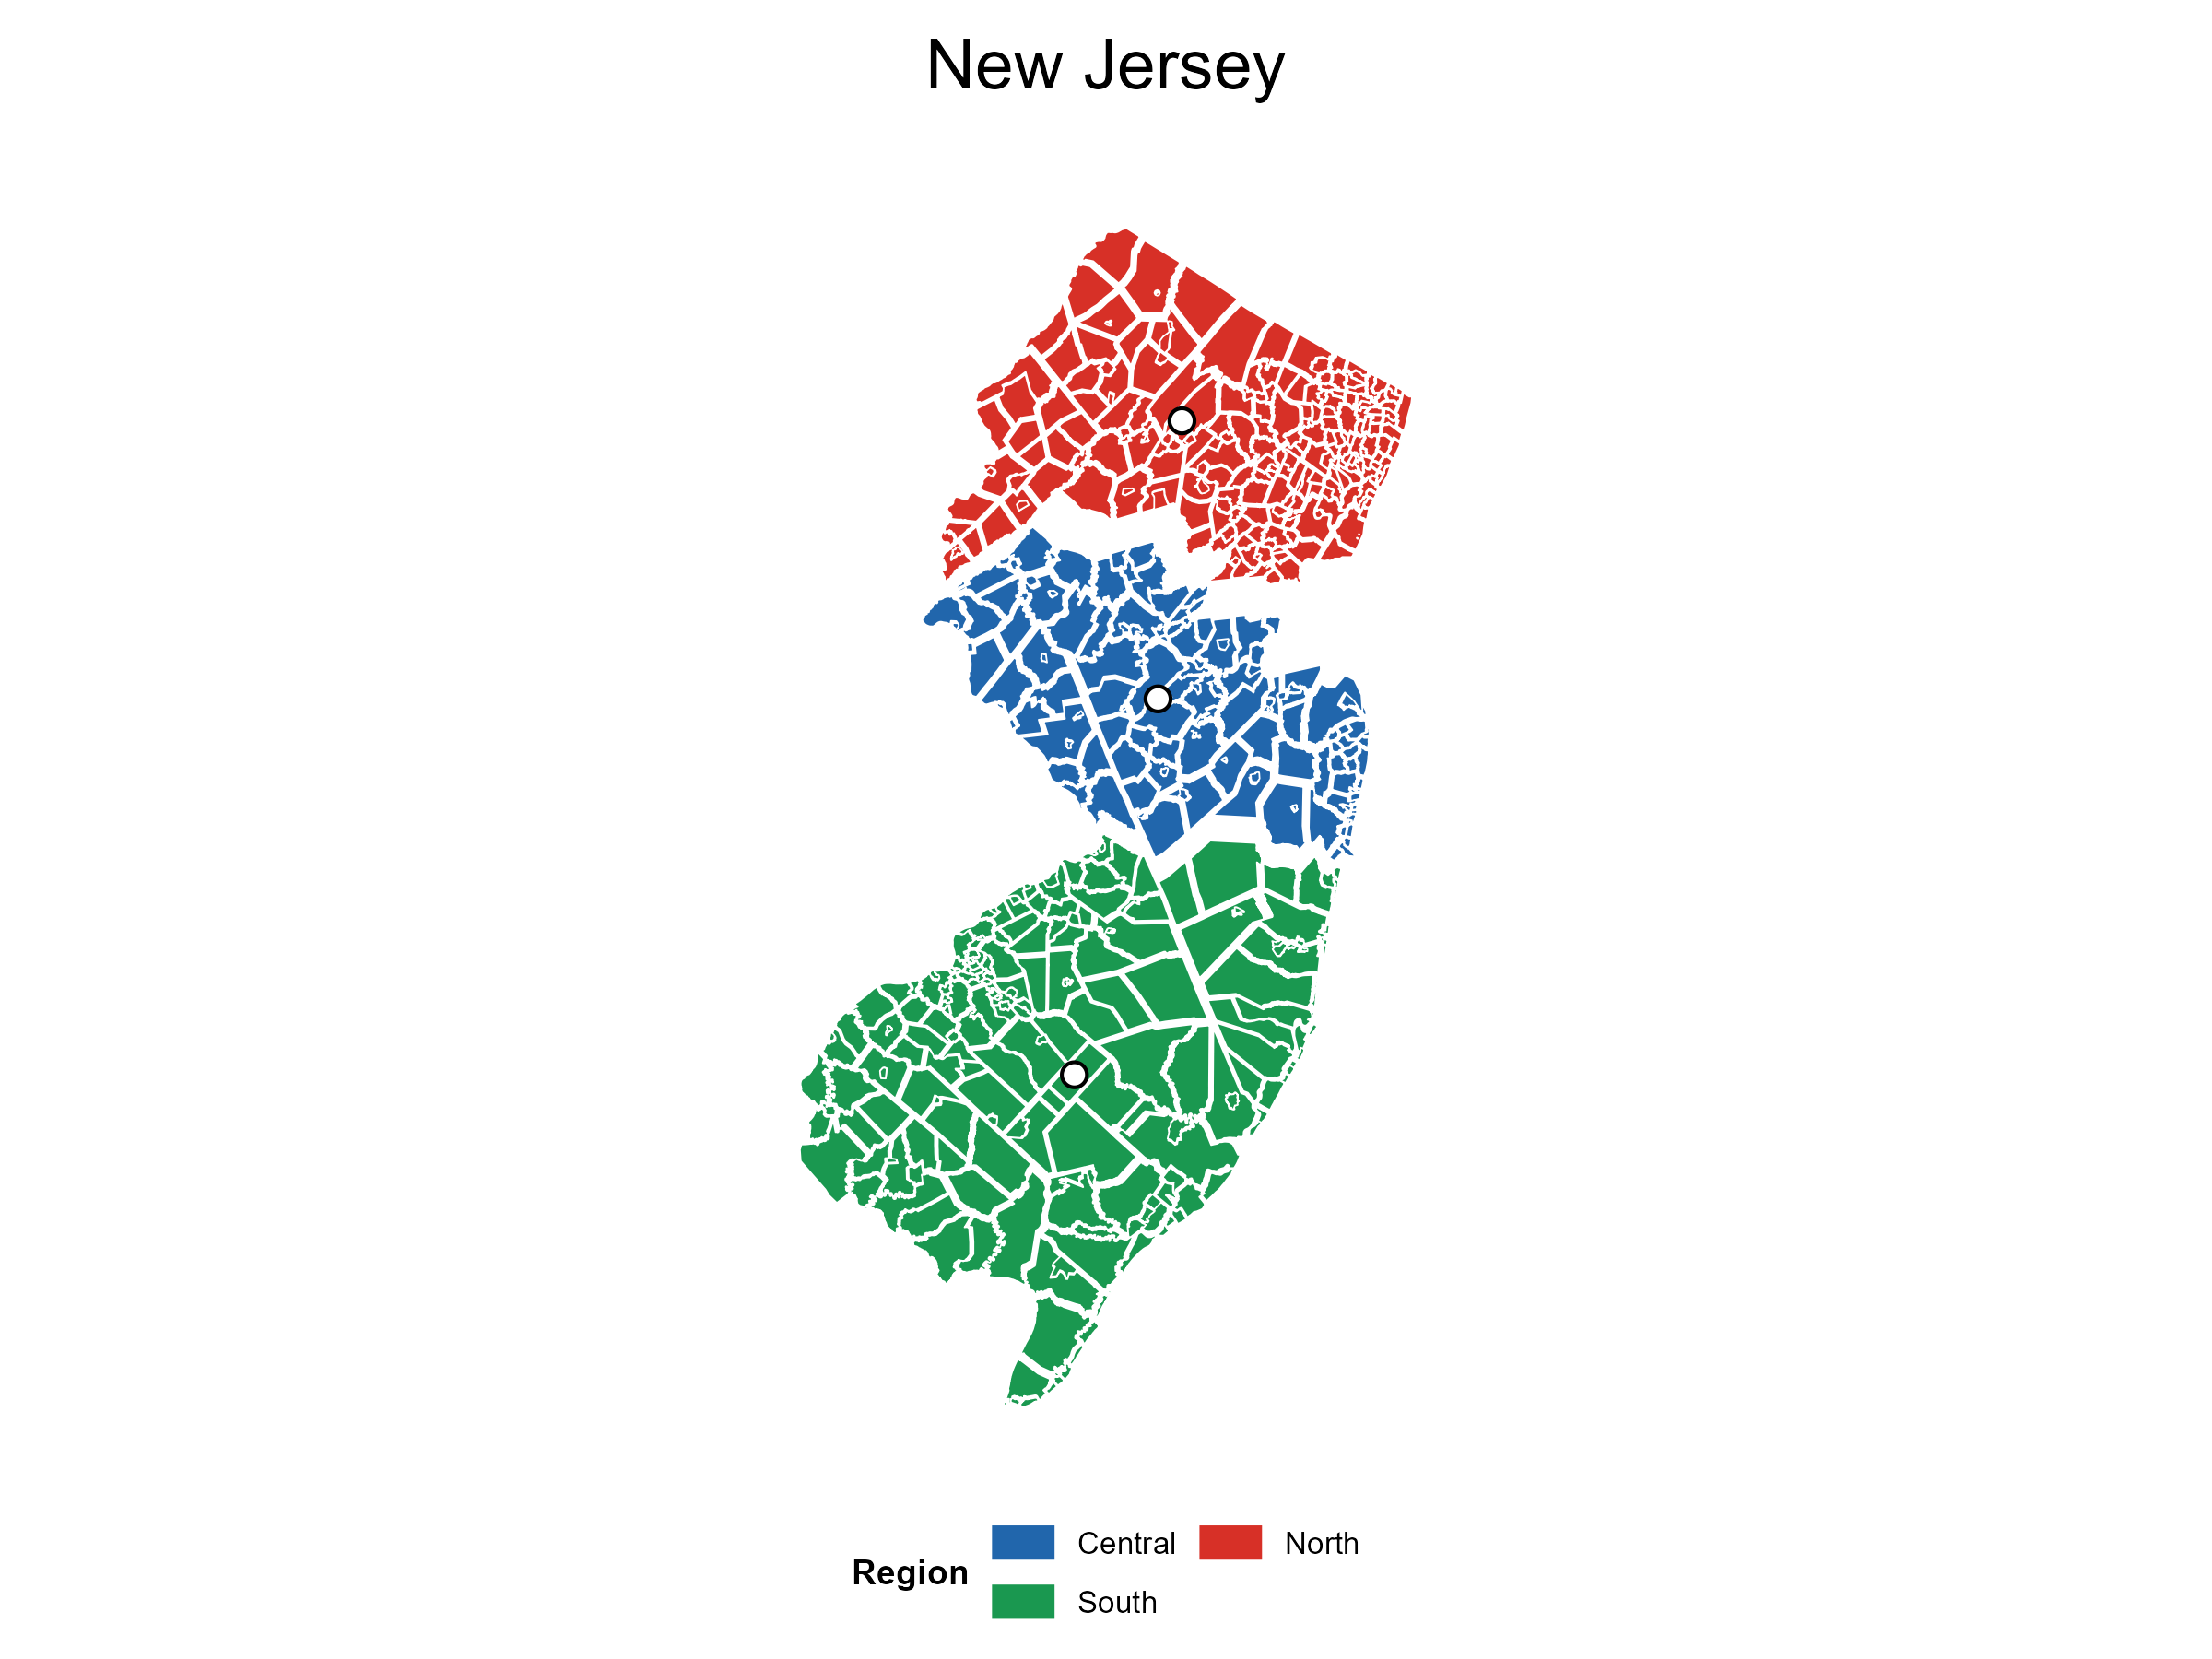
\includegraphics[width=0.72\textwidth]{nj_dragged_layout.png}
\caption{Formula-derived output plus documented display offsets: New Jersey municipalities ($n = 564$) using the calibrated displacement values and display offsets stored in \texttt{paper/outputs/tables/nj\_drag\_offsets.csv}. North, Central, and South regions are separated by the regional displacement term while each municipality's internal geometry is preserved exactly. Quantitative metrics use the analytical output before these display offsets unless explicitly stated otherwise.}
\label{fig:nj_exploded}
\end{figure}

% ─────────────────────────────────────────────────────────────────────────────
\section{Cross-State Transfer Test: Pennsylvania}
% ─────────────────────────────────────────────────────────────────────────────

\subsection{Dataset and Motivation}

To evaluate the robustness of the derived parameter structure, the method was applied to municipal boundary data from Pennsylvania. The Pennsylvania dataset contains 2{,}572 municipalities across six macro-regions, representing a substantially larger and more heterogeneous administrative structure than the New Jersey case study. Pennsylvania provides a demanding transfer test: 4.5$\times$ more administrative units, a state approximately 3$\times$ larger in area, and two competing high-density cores (Philadelphia and Pittsburgh) separated by extensive rural terrain.

\subsection{Regional Hierarchy}

Counties were assigned to six macro-regions: Southeast (5 counties, Philadelphia metro), Northeast (15 counties, Poconos and Lehigh Valley), Central (15 counties, rural spine), SouthCentral (12 counties, Harrisburg--Lancaster corridor), Southwest (10 counties, Pittsburgh metro), and Northwest (10 counties, Erie and Oil Country).

\subsection{Transfer Results}

Parameters $\gamma_r$ and $\gamma_l$ estimated from the New Jersey dataset were applied directly without additional tuning. Applying the geometry-derived formulas to the PA geometry ($\bar{w} = 6{,}725$\,m, $n_r = 6$, $\widetilde{R}_{\text{local}} = 116{,}086$\,m, $\bar{n} = 449$) yields $\alpha_r = 20{,}174$\,m and $\alpha_l = 12{,}447$\,m. These values are consistent with the cross-state calibration table (Table~\ref{tab:crossstate}). A focused sensitivity analysis varying $\alpha_l$ by $\pm 15\%$ around the formula-derived value showed smooth variation in mean displacement (CV $< 0.02$) and mean neighbor gap across all levels, supporting the formula-derived value as a reproducible starting point.

Note that Pennsylvania serves a dual role in the analysis: it tests transferability of the NJ-calibrated $\gamma_l$, and it provides an \emph{indicative} second regional coefficient rather than a final independent visual-reference calibration, since earlier PA visual values were partially heuristic. The resulting displacement produced a usable six-region layout while preserving recognizable geographic structure, but residual tight spacing remains in the densest metro cores (Section~\ref{sec:evaluation}).

\subsection{Density Asymmetry and the $s_i$ Term}

The Southwest region (Pittsburgh metro) contains 551 municipalities across 10 counties, while the Southeast region (Philadelphia metro) contains 239 across 5. Both exhibit extreme municipal density near their regional centroids. The diagnostic vector-field visualization shows that the distance-scaling coefficient $s_i$ suppresses displacement in both cores while allowing full expansion at regional peripheries---the intended behavior of Equation~\eqref{eq:si}.

\subsection{Properties Demonstrated}

The Pennsylvania experiment demonstrates three important properties of the framework:

\begin{description}
  \item[Scalability.] The closed-form displacement step handled more than four times the number of administrative units present in the New Jersey dataset without performance degradation, consistent with $O(n)$ behavior in feature count.
  \item[Parameter transferability.] Applying the NJ-calibrated coefficient $\gamma_l = 1.136$ to Pennsylvania yields $\alpha_l = 12{,}447$\,m. Sensitivity analysis across a $\pm 15\%$ range shows smooth changes in mean displacement and mean neighbor gap at all tested levels. The formula-derived value is substantially smaller than the heuristic value of 40{,}000\,m used in initial PA runs, indicating that the heuristic over-expanded municipalities locally. The formula-derived value is the recommended analytical starting parameter for PA deployment.
  \item[Hierarchical flexibility.] The same displacement model was applied across both a small dense state and a large heterogeneous one, demonstrating applicability across geographic scale and administrative density.
\end{description}

The PA value $\widetilde{R}_{\text{local}}/\bar{w} = 17.26$ remains close to the NJ value of 15.83, indicating that both states belong to the same fine-grained municipal regime identified in the broader cross-state validation (Section~\ref{sec:ratio}).

\begin{figure}[H]
\centering
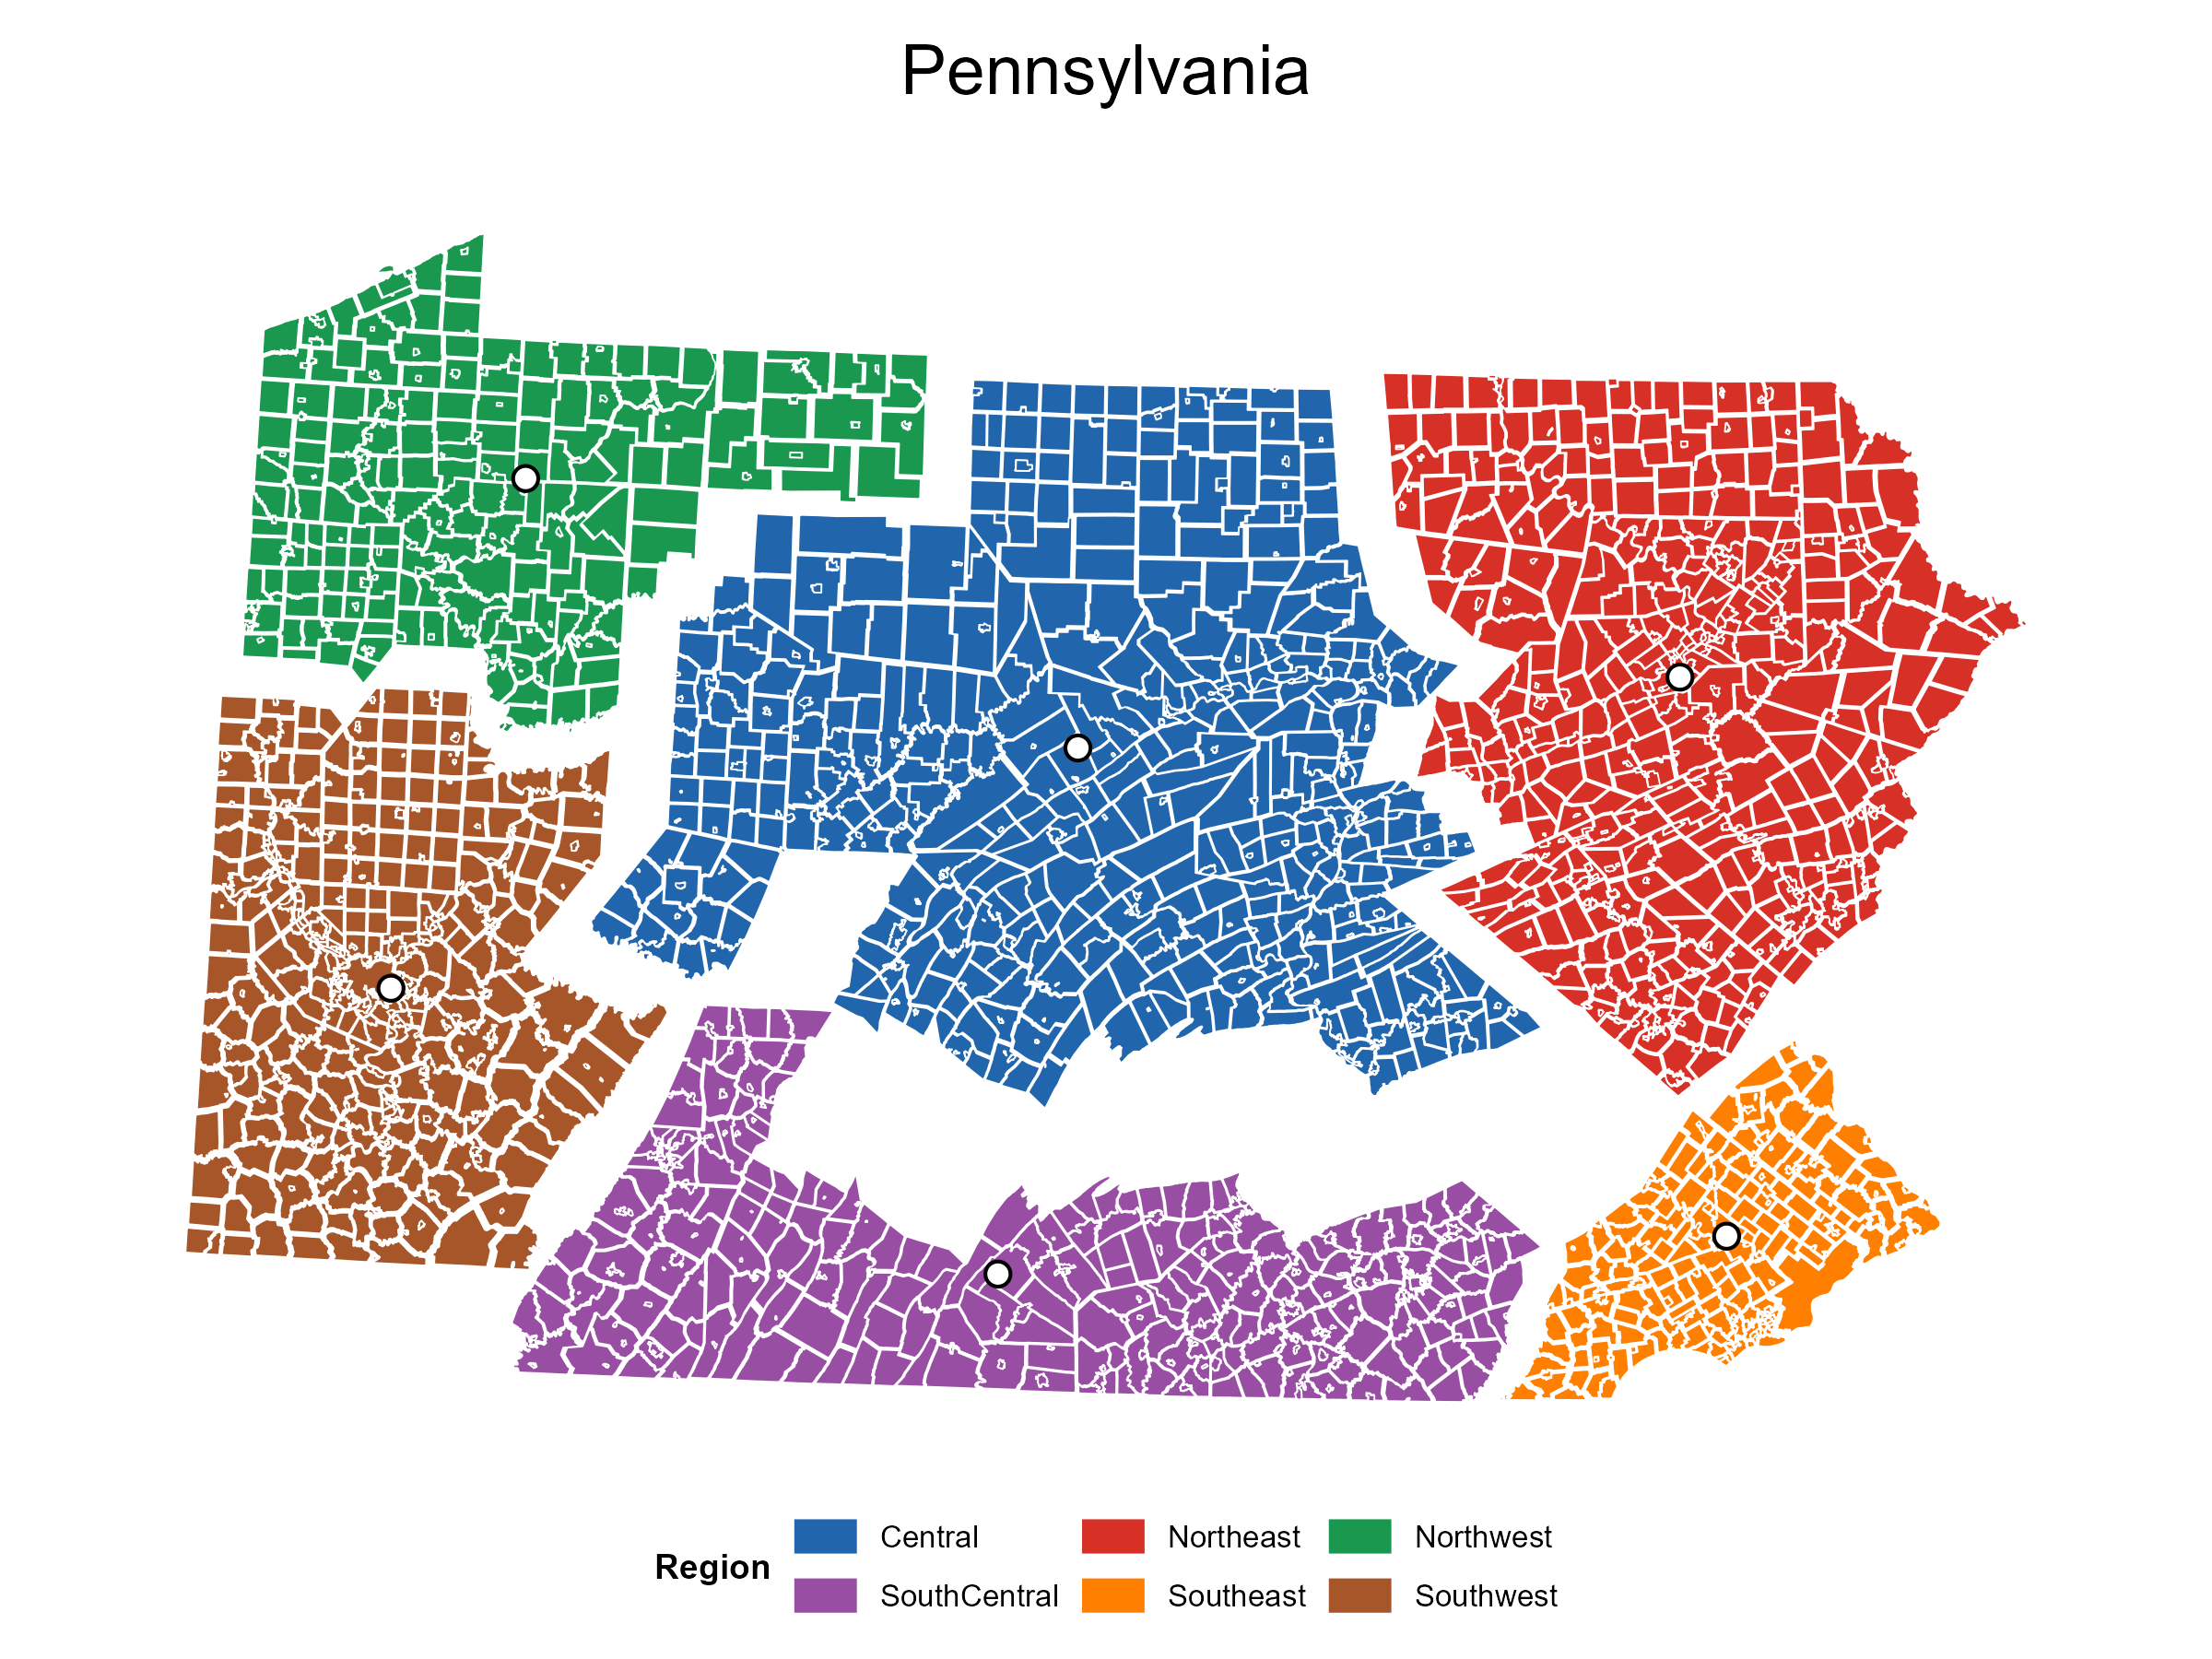
\includegraphics[width=0.92\textwidth]{pa_dragged_layout.png}
\caption{Formula-derived output plus documented display offsets: Pennsylvania municipalities ($n = 2{,}572$) after analytical displacement ($\alpha_r = 20{,}174$\,m, $\alpha_l = 12{,}447$\,m, $p = 1.25$) and region-level display offsets. The offsets are rigid translations recorded in \texttt{paper/outputs/tables/pa\_drag\_offsets.csv}; they improve figure composition without changing any municipality's shape, area, or within-region relative arrangement.}
\label{fig:pa_exploded}
\end{figure}

% ─────────────────────────────────────────────────────────────────────────────
\subsection{Documented Display Offsets}
\label{sec:displayoffsets}

The formula-derived displacement produces the analytical layout used for validation. For final paper figures, a second reproducible display step may apply small rigid translations to whole parent regions to improve composition, reduce page whitespace, and avoid label collisions. These offsets do not alter the displacement model itself: every child feature in a region receives the same additional vector, so shape, area, orientation, and within-region relative geometry remain unchanged.

The display offsets used in this paper were selected with an interactive drag helper and saved as CSV files with columns \texttt{region}, \texttt{dx\_m}, and \texttt{dy\_m}. The package function \texttt{apply\_region\_offsets()} applies these tables to raw \texttt{sf}, \texttt{exploded\_map}, or \texttt{grouped\_exploded\_map} objects. This separates analytical parameter validation from cartographic finishing and makes all manual figure adjustments auditable.

\section{Diagnostic Analysis}
\label{sec:diagnostic}
% ─────────────────────────────────────────────────────────────────────────────

\subsection{Displacement Vector Field}

To validate the method, a displacement vector field was constructed from municipality centroids:
\begin{equation}
  t_i = C'_i - C_i
  \label{eq:diag}
\end{equation}
where $C_i$ and $C'_i$ are the original and displaced centroids respectively. This diagnostic is formally equivalent to the cartographic deformation field analysis described in \citet{jenny2011}.

\subsection{Interpretation}

The resulting vector field demonstrates three expected properties:
\begin{enumerate}
  \item \textbf{Coherent outward radial displacement} within each region, confirming correct orientation of the local unit vector field.
  \item \textbf{Larger displacement magnitudes} near regional boundaries, where the local component $s_i\,\hat{d}_{\text{local},i}$ is greatest.
  \item \textbf{Reduced displacement near regional centroids}, confirming that $s_i$ suppresses void formation without post-hoc correction.
\end{enumerate}

These properties are consistent with geographically coherent displacement behavior predicted by the theoretical structure of $V(x) = V_{\text{region}}(x) + V_{\text{local}}(x)$. The outward radial structure is a diagnostic check on Proposition~2: because $s_i$ is monotonic in $\|C_i - C_r\|$, units retain their radial ordering after displacement, and the vector field reflects this as smooth outward expansion rather than crossing or disordering of displacement directions.

\begin{figure}[H]
\centering
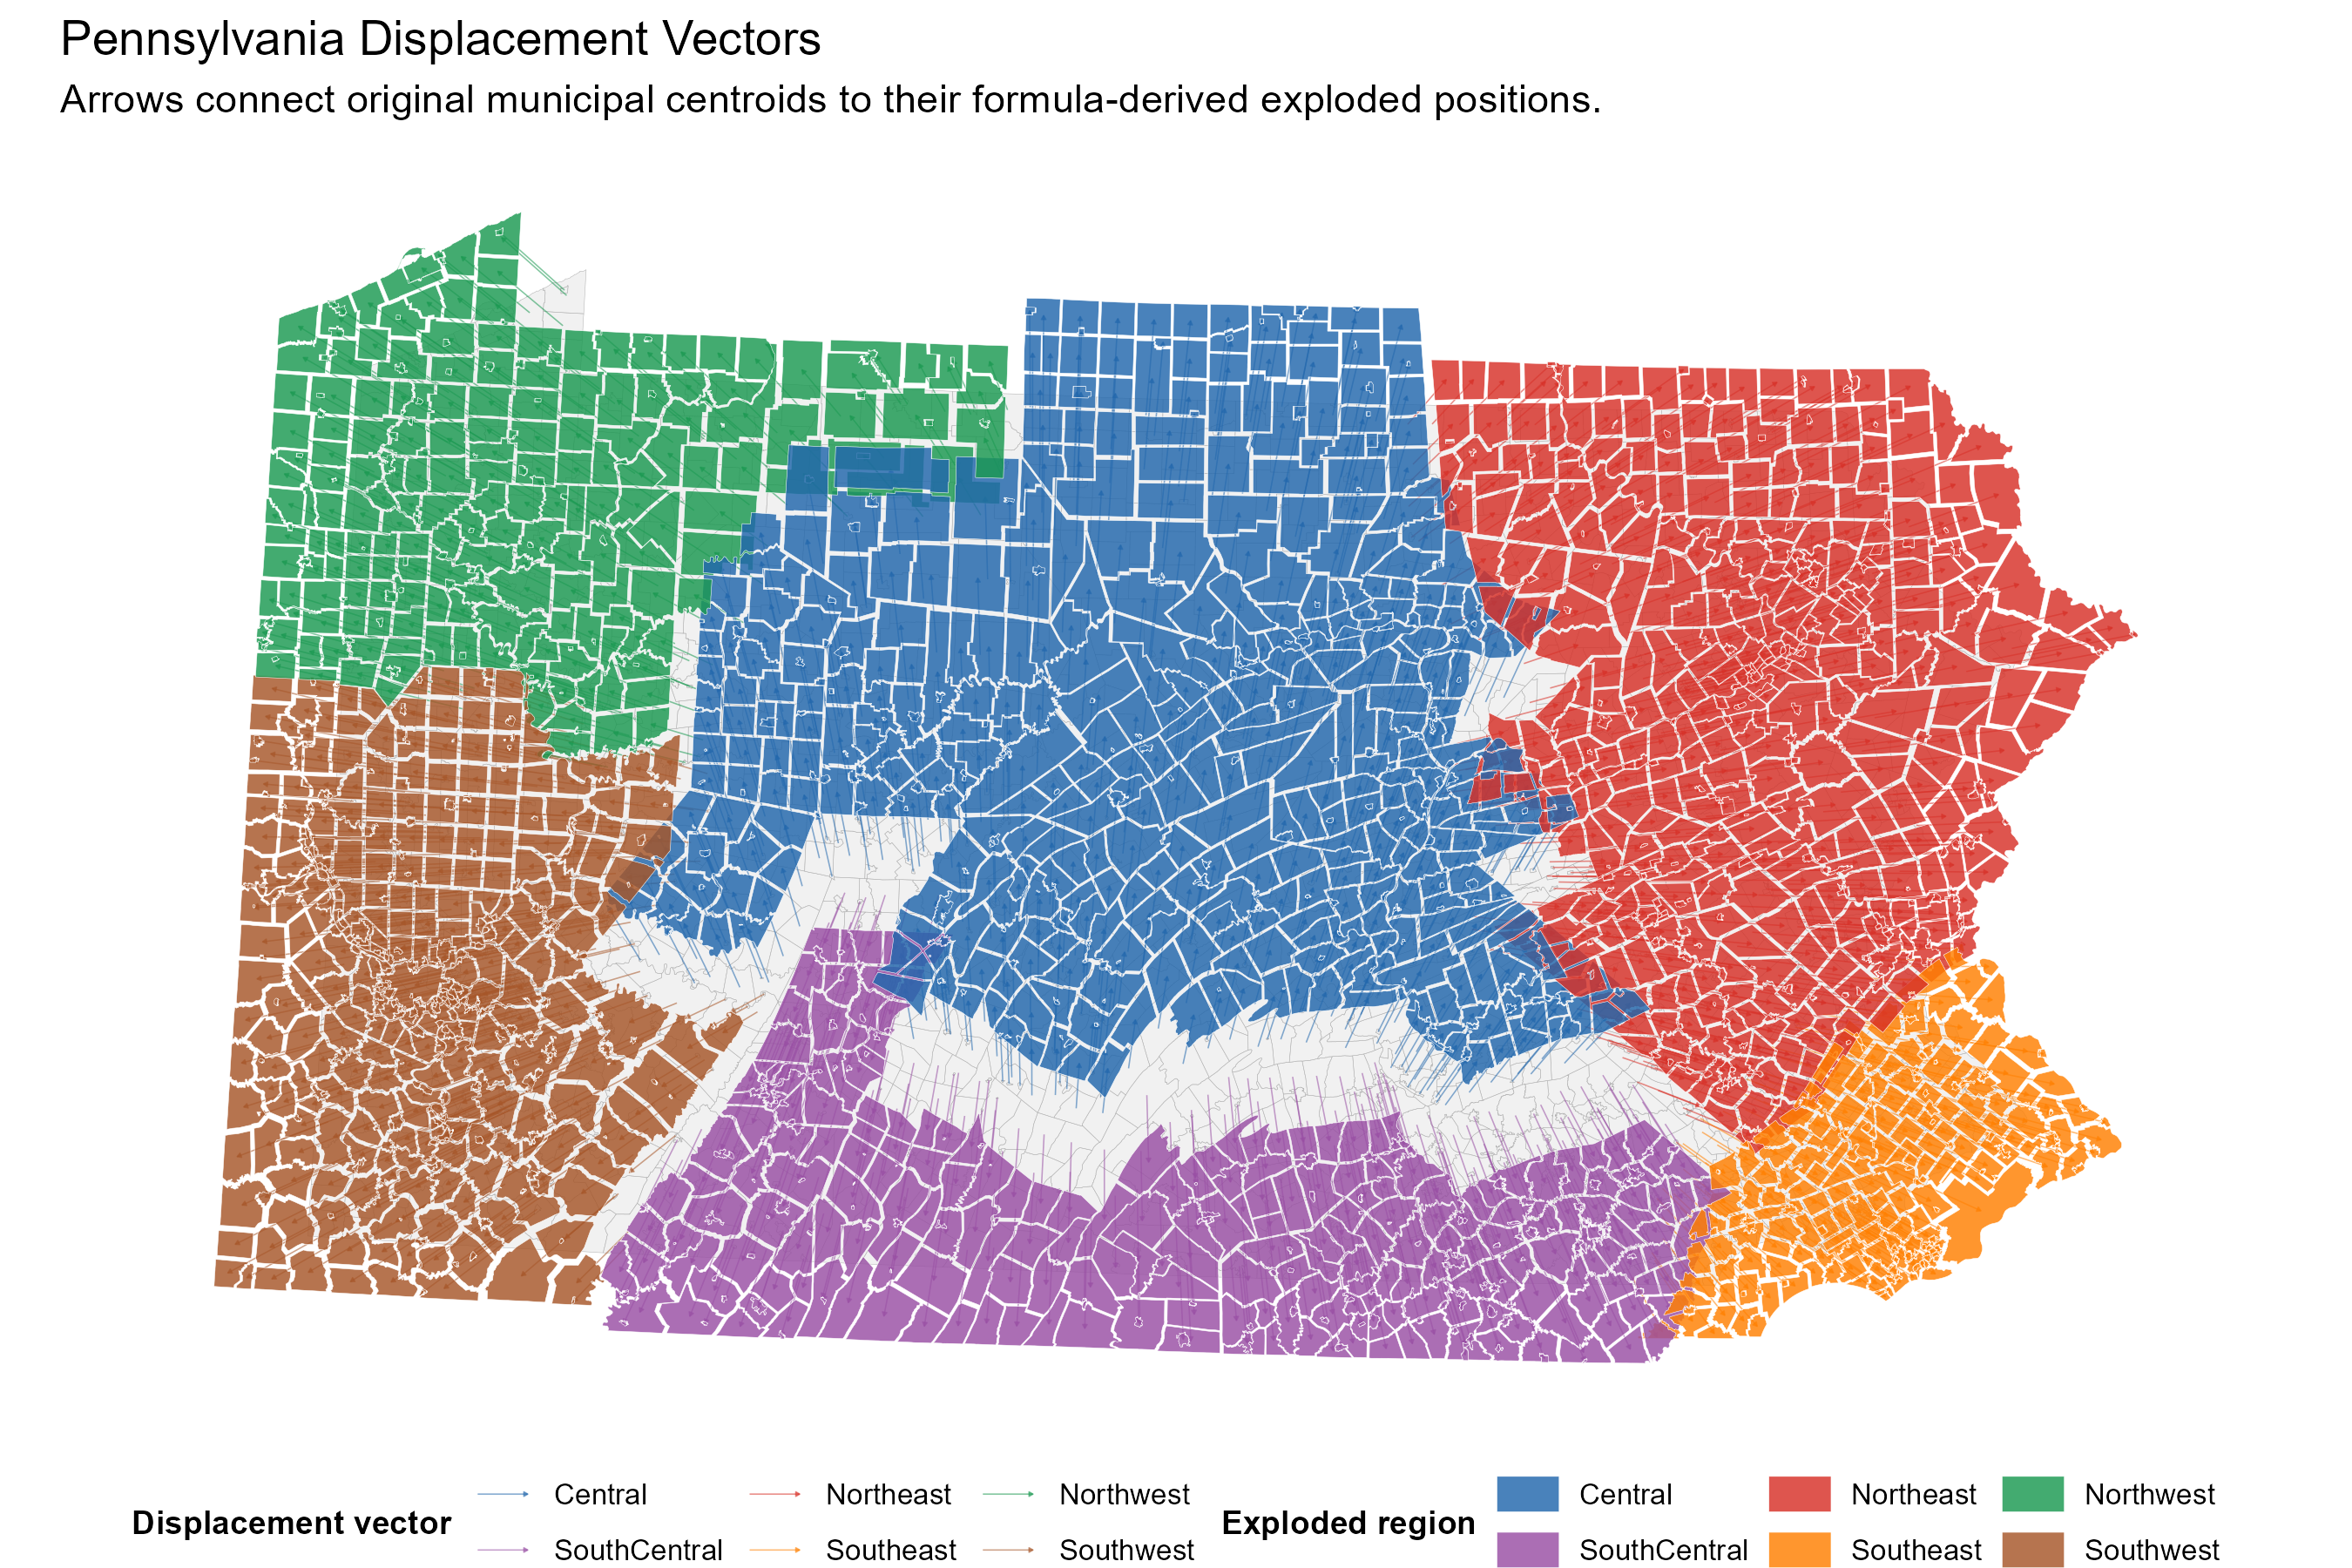
\includegraphics[width=0.92\textwidth]{pa_displacement_vectors.png}
\caption{Diagnostic comparison: Pennsylvania displacement vector field. Grey polygons show the original municipal coverage, coloured polygons show the formula-derived analytical exploded layout before display offsets, and arrows connect each municipality's original centroid to its analytical exploded centroid. The figure visualizes how the regional and local displacement terms pull municipalities apart while preserving each polygon by rigid translation.}
\label{fig:pa_vectors}
\end{figure}


% ─────────────────────────────────────────────────────────────────────────────
\section{Discussion}
\label{sec:discussion}
% ─────────────────────────────────────────────────────────────────────────────

The method occupies a middle ground between classical displacement operators and continuous deformation models. Like displacement methods, it improves readability by introducing whitespace. Like cartograms and deformation approaches, it may be understood as a transformation field over the map domain. Unlike both, it preserves each polygon's interior geometry exactly through rigid-body translation (Proposition~1), while the displacement step remains analytically closed-form and $O(n)$ in feature count.

\subsubsection*{Preservation guarantees}

The following distinction is precise and important. \emph{Internally}, each administrative unit is transformed by rigid motion: its shape, area, perimeter, orientation, and topological structure are all preserved exactly. \emph{Globally}, the method does not guarantee preservation of adjacency or shared-boundary coincidence among distinct units after displacement. Neighboring municipalities that shared a boundary before explosion will generally have a gap between them afterward. This is by design in the exploded-view context --- the introduction of whitespace is the goal --- but it means the output should not be treated as a topologically consistent coverage.

\begin{table}[h]
\centering
\caption{Comparison of method classes on key cartographic properties.}
\label{tab:comparison}
\begin{adjustbox}{max width=\textwidth}
\begin{tabular}{lccc}
\toprule
\textbf{Property} & \textbf{Optimization displacement} & \textbf{Cartogram / deformation} & \textbf{This method} \\
\midrule
Feature shape preserved   & Partial        & No             & \textbf{Yes (exact)} \\
Feature area preserved    & Partial        & No (by design) & \textbf{Yes (exact)} \\
Adjacency preserved       & Yes (goal)     & Partial        & No (by design) \\
Continuous deformation    & No             & Yes            & No \\
Piecewise rigid motion    & No             & No             & \textbf{Yes} \\
Closed-form               & No             & No             & \textbf{Yes} \\
$O(n)$ complexity         & No             & No             & \textbf{Yes} \\
Hierarchy-aware           & Rarely         & Rarely         & \textbf{Yes} \\
\bottomrule
\end{tabular}
\end{adjustbox}
\end{table}

\subsubsection*{Limitations and future work}

The method does not guarantee positive inter-unit spacing for all displaced unit pairs. As demonstrated in Section~\ref{sec:evaluation}, residual contact at formula-derived parameters is primarily density-driven: in compact high-density regions such as the Philadelphia metro core, the formula-derived $\alpha_l$ produces uniformly tight spacing throughout the region, with contact cases distributed across the full $s_i$ range rather than confined to centroid-proximate units. The natural extension is a two-stage hybrid pipeline: the closed-form analytical displacement (Algorithm~1) serves as Stage~1, producing a hierarchy-respecting, radially coherent layout within a bounded displacement envelope; a local collision-refinement stage then resolves residual spacing violations for units whose post-explosion gap falls below a user-specified threshold. Such a refinement would modify only units involved in spacing conflicts, preserve geometry exactly (because corrections remain rigid translations), stay close to the analytical displacement field, and exploit the bounded-displacement guarantee of Proposition~3 to constrain the refinement search space.

The zoom-dependent extension $t_i(z) = \lambda(z) \cdot t_i$ (Equation~\ref{eq:zoom}) is particularly promising for interactive web maps, where smooth explosion and collapse can serve both overview and detail display modes from a single dataset without geometry duplication.

The \texttt{explodemap} package also includes \texttt{focus\_map()}, an interactive \textsf{R}/htmlwidgets companion for inspecting dense administrative maps in Shiny applications. This widget should be distinguished from the exploded-view transformation studied in this paper. The exploded map changes feature locations in projected map coordinates through the displacement field $G'_i = G_i + t_i$. By contrast, \texttt{focus\_map()} operates primarily in viewport coordinates: a selected feature is fit to a target screen fraction, optionally lifted for emphasis, and accompanied by a non-blocking information card. The selected feature's underlying geographic geometry is not re-estimated by the focus interaction. Its mathematical object is therefore a view transform and screen-space emphasis model rather than a new cartographic displacement field. A separate companion manuscript develops this focus-map interaction model, including selected-feature viewport fitting, label visibility thresholds, and dense-layer rendering heuristics.

\subsubsection*{Mathematical classification}

From a mathematical perspective, the transformation defined here may be characterized as a \emph{hierarchical piecewise-rigid displacement field over a polygonal partition of the plane}. As established in Section~3.6, the executed field $V(x) = t_i$ is constant within each polygon domain $G_i$ (Equation~\eqref{eq:piecewise}), making the transformation piecewise rigid by construction. The method samples smooth radial potentials at the unit-centroid level, then executes the sampled displacement as a piecewise-constant rigid translation over each polygon. The resulting field is therefore not globally continuous; its discontinuities occur at polygon boundaries, where whitespace is intentionally introduced.

\subsubsection*{Scalar potential representation}

Within each parent region, the generating displacement field admits a compact scalar potential representation. Let $r(x) = \|x - C_r\|$ denote the distance from an arbitrary point $x$ to the region centroid. Since the regional direction $\hat{d}_{\text{state},r}$ is inherited from the parent-region centroid and is constant within region $r$, and since $\nabla r(x) = \hat{d}_{\text{local}}$, the two displacement components can be written as gradients:
\[
  \alpha_r\,\hat{d}_{\text{state},r} = \nabla\!\left(\alpha_r\,\hat{d}_{\text{state},r}\cdot x\right), \qquad
  \alpha_l\,s_i\,\hat{d}_{\text{local}} = \nabla\!\left(\frac{\alpha_l}{(p+1)\,d_{\max,r}^p}\,r(x)^{p+1}\right).
\]
The full generating field within region $r$ is therefore $V(x) = \nabla\Phi_r(x)$, where the scalar potential is:
\begin{equation}
  \Phi_r(x) = \alpha_r\,\hat{d}_{\text{state},r}\cdot x + \frac{\alpha_l}{(p+1)\,d_{\max,r}^p}\,r(x)^{p+1}.
  \label{eq:potential}
\end{equation}
The first term is a \emph{linear directional potential} with constant gradient $\alpha_r\,\hat{d}_{\text{state},r}$; the second is a \emph{local superlinear radial potential} centred on the region centroid. The exponent $p+1 > 2$ in the local term directly explains why outer units expand more strongly than inner ones while preserving radial ordering (Proposition~2): the local potential grows superlinearly with distance from $C_r$, so its gradient — the displacement magnitude — increases monotonically with $r(x)$.

The centroid-driven displacement vectors may therefore be interpreted as samples from a hierarchical radial potential field, executed through piecewise rigid translations rather than continuous deformation. This is the precise sense in which the method is a \emph{hierarchical radial expansion transform}. To be explicit: $\Phi_r(x)$ describes the \emph{generative} field --- a continuous scalar potential from which displacement directions and magnitudes are derived --- while the \emph{executed} map transformation remains piecewise rigid over polygons, with each unit receiving a single constant translation vector sampled from this field at its centroid.

This combination --- continuous generative potential, piecewise rigid execution, exact geometry preservation --- differentiates the method from three common families of cartographic transformation (rigid transforms, continuous deformation, and topological rearrangement). Analyzing the theoretical properties of this formulation --- conditions for guaranteed non-overlap, stability under repeated application, and bounds on feature separation as a function of the potential parameters --- represents a natural direction for future work.

% ─────────────────────────────────────────────────────────────────────────────
\section{Applications}
% ─────────────────────────────────────────────────────────────────────────────

Because the displacement step is deterministic, $O(n)$ in feature count, and operates directly on vector geometries, it is well suited for:
\begin{itemize}
  \item exploded choropleth and thematic administrative maps,
  \item interactive municipal dashboards with hover, click, and tooltip interactions,
  \item multi-scale cartographic exploration via zoom-dependent explosion,
  \item educational and journalistic cartography with animated transitions,
  \item real-time Shiny and web-map interfaces with live parameter adjustment,
  \item interactive focus-map inspection workflows in which users select an administrative unit, zoom to a legible viewport target, and read contextual attributes in a non-blocking card.
\end{itemize}

\subsection{Generalized Implementation}
\label{sec:genimpl}

A key practical contribution is a generalized open implementation in the \texttt{explodemap} \textsf{R} package. The package exposes three entry points depending on how the practitioner's data is organized. The reference implementation is a direct software realization of Algorithm~1; only the data-ingestion and grouping interface differ across entry points.

\begin{description}
  \item[\texttt{explode\_state(fips, crs, region\_map)}] Downloads U.S.\ Census TIGER/Line 2024 county subdivision boundaries automatically for a given state, attaches user-defined region labels via county name lookup, derives parameters using Analytical Results~1 and~2, and returns original and exploded \texttt{sf} objects with GeoJSON export. A disk-based cache prevents redundant downloads across sessions.

  \item[\texttt{explode\_sf(sf\_obj, region\_col)}] Accepts any projected \texttt{sf} object that already has a grouping column attached --- whether from a local shapefile, a database query, or a spatial join. Works with any polygon dataset at any administrative scale: census tracts, school districts, watersheds, electoral constituencies, or custom analytical regions.

  \item[\texttt{explode\_sf\_with\_lookup(sf\_obj, join\_col, lookup)}] Joins an external lookup table (CSV, data frame, or database result) to the \texttt{sf} object before exploding, enabling groupings that are defined outside the spatial data itself --- for example, grouping municipalities by political party, by health service area, or by any non-geographic classification.
\end{description}

All three entry points use the same core \texttt{explode\_map} algorithm (Algorithm~1) and the same parameter derivation procedure (Analytical Results~1--2), ensuring that the mathematical guarantees of Propositions~1--3 apply uniformly regardless of how the data is supplied. This enables direct application of the framework to any polygonal partition with a defined grouping, allowing users to ``explode'' arbitrary spatial hierarchies without modification to the underlying algorithm. The generalized implementation exposes the same core mathematical transformation described in Algorithm~1; only the data-ingestion and grouping interface change across entry points.

% ─────────────────────────────────────────────────────────────────────────────
\section{Quantitative Evaluation}
\label{sec:evaluation}
% ─────────────────────────────────────────────────────────────────────────────

Although exploded cartographic layouts are primarily assessed through visual inspection, several quantitative indicators characterize the behavior and correctness of the displacement framework.

\subsection{Computational Complexity}

The displacement step is $O(n)$ in the number of administrative units. Each unit requires a fixed number of centroid and vector computations independent of all other units. No iterative passes, energy minimization, or topology reconstruction are required in this step. End-to-end runtime also includes geometry preprocessing, CRS transformation, unions, centroid calculations, plotting, and optional refinement; Table~\ref{tab:crossstate} reports observed runtimes for the reproducible cases.

\subsection{Geometric Fidelity}

By Proposition~1 (Section~3.2), translation is a Euclidean isometry: every polygon is transformed by $G'_i = G_i + t_i$, preserving all interior distances, areas, angles, and topological structure exactly. The internal polygon distortion induced by the method is zero by construction. This is a strict guarantee, not an approximation, and holds regardless of parameter values or the size of the displacement vectors.

\subsection{Parameter Calibration Fit}

For the New Jersey case study, where manual visual reference values are available, the geometry-derived formulas produce the following calibration fits under working defaults ($\gamma_r = 3.0$, $\gamma_l = 1.136$):

\begin{center}
\begin{tabular}{lrrl}
\toprule
\textbf{Parameter} & \textbf{Manual} & \textbf{Derived} & \textbf{Error} \\
\midrule
$\alpha_r$ & 6{,}000\,m  & 6{,}832\,m  & $+13.8\%$ \\
$\alpha_l$ & 10{,}000\,m & 10{,}001\,m & $<0.1\%$  \\
\bottomrule
\end{tabular}
\end{center}

The $\alpha_l$ value is an exact calibration fit for the NJ reference layout because $\gamma_l$ is estimated from that same reference. It should not be interpreted as independent prediction accuracy. The $\alpha_r$ difference of 13.8\% reflects residual uncertainty in $\gamma_r$, which has not yet been stabilized across a sufficient number of independent visual reference cases. In practice, an $\alpha_r$ difference of this magnitude produces a useful starting layout that may require documented display offsets or additional calibration of regional spacing.

\subsection{Displacement Field Diagnostics}

The diagnostic displacement vector field (Section~\ref{sec:diagnostic}) shows three expected structural properties across both case studies: outward radial orientation within each region, larger displacement magnitudes near regional peripheries, and suppressed displacement near regional centroids consistent with the $s_i$ weighting function. These properties hold in both the three-region NJ configuration and the six-region PA configuration, indicating that the vector field structure behaves consistently under variation in regional count and geographic extent.

\subsection{Minimum Inter-Unit Spacing}

A direct measure of the whitespace introduced by the algorithm is the minimum inter-unit spacing $d_{\min}$, defined as:
\[
  d_{\min} = \min_{i \neq j}\, \mathrm{dist}(G'_i,\, G'_j)
\]
where $\mathrm{dist}(G'_i, G'_j)$ is the minimum boundary-to-boundary Euclidean distance between distinct exploded units $i$ and $j$, computed in the projected working CRS with linear metre units. In the original geographic layout, adjacent municipalities share boundaries as cells of a contiguous administrative coverage, so $d_{\min} = 0$ by definition --- the pre-explosion minimum is necessarily zero. The post-explosion nonzero minimum is therefore a direct indicator of the whitespace creation that is the method's primary purpose.

\begin{table}[h]
\centering
\caption{Minimum and mean inter-unit spacing and mean displacement magnitude before and after explosion. Mean neighbor gap is defined as the mean nearest-boundary Euclidean distance between each unit and its closest distinct neighbor in the exploded layout, computed in the projected working CRS. Mean $\|t_i\|$ is the arithmetic mean of displacement vector magnitudes across all units.}
\label{tab:dmin}
\begin{adjustbox}{max width=\textwidth}
\begin{tabular}{lrrrrrr}
\toprule
\textbf{Dataset} & \textbf{$n$} & \textbf{$d_{\min}$ (pre)} & \textbf{$d_{\min}$ (post)} & \textbf{Mean neighbor gap} & \textbf{Mean $\|t_i\|$} \\
\midrule
NJ ($\alpha_r=6{,}000$, $\alpha_l=10{,}000$)   & 564   & 0\,m & $\approx 1{,}200$\,m & $\approx 4{,}800$\,m & $\approx 7{,}300$\,m \\
PA ($\alpha_r=20{,}174$, $\alpha_l=12{,}447$)  & 2{,}572 & 0\,m & 0\,m$^{\dagger}$ & $\approx 67$\,m & $\approx 20{,}630$\,m \\
\bottomrule
\end{tabular}
\end{adjustbox}
\end{table}

$^{\dagger}$At formula-derived parameters, the minimum spacing is zero for adjacent units in dense regions. Three observations characterize the spacing behavior. First, mean separation improves: the mean neighbor gap is positive for both datasets, confirming that the analytical field introduces whitespace across a substantial fraction of the layout. Second, inter-region separation is strong: the regional displacement term $\alpha_r$ cleanly separates parent regions, and peripheral municipalities within each region receive proportionally larger local displacement via the $s_i$ weighting. Third, worst-case minimum spacing is not guaranteed and is not confined to centroid-proximate units: in compact high-density regions such as the Philadelphia metro core (239 municipalities in 5 counties), 65.7\% of unit pairs remain within 50\,m of a neighbor after explosion, with contact cases distributed across the full $s_i$ range rather than concentrated at $s_i \approx 0$. This indicates that the residual contact is density-driven --- the formula-derived $\alpha_l$ is structurally appropriate for the state as a whole but modest relative to the extreme density within the most compact region.

\medskip
\noindent The method does not guarantee global non-overlap at formula-derived parameters. Explicit collision detection to guarantee a user-specified $d_{\min}$ threshold across all unit pairs remains a direction for future work; the bounded-displacement property (Proposition~3) ensures that any such refinement operates within a known envelope of radius $\alpha_r + \alpha_l$.

\medskip
\noindent The current sensitivity analysis is intentionally narrow: it reports mean displacement and mean neighbor-gap behavior around the Pennsylvania formula-derived $\alpha_l$. A complete validation benchmark should also vary $\alpha_r$, $\alpha_l$, and $p$ jointly and report worst-case spacing, median nearest-neighbor gap, percent of units below a spacing threshold, residual contact counts, maximum displacement, and regional localization of failures. The present manuscript therefore treats the Pennsylvania sensitivity result as evidence of smooth parameter response, not as proof that the formula-derived layout optimizes dense-core clearance.

% ─────────────────────────────────────────────────────────────────────────────
\section{Extended Evaluation: Additional U.S. States, Canada, and Germany}
\label{sec:extended}
% ─────────────────────────────────────────────────────────────────────────────

Additional cases were selected for extended evaluation targeting structural properties that the New Jersey and Pennsylvania case studies do not fully exercise. Ohio and Michigan test dense municipal systems with different regional geometries; Kentucky, Illinois, North Dakota, North Carolina, Virginia, Texas, and Florida broaden the U.S.\ comparison; Canada and Germany test reproducibility beyond a single U.S.\ administrative context.

\begin{table}[H]
\centering
\caption{Validation tiers used in the manuscript.}
\label{tab:validation_tiers}
\begin{adjustbox}{max width=\textwidth}
\begin{tabular}{lll}
\toprule
\textbf{Tier} & \textbf{Cases} & \textbf{Evidence type} \\
\midrule
Calibration and transfer case studies & New Jersey, Pennsylvania & Parameters, spacing metrics, displacement diagnostics, display-offset audit \\
Structural stress tests & Ohio, Michigan, Canada & Formula-derived parameters, tightness ratios, static outputs, diagnostic interpretation \\
Broad reproducibility tests & Illinois, North Dakota, North Carolina, Kentucky, Virginia, Texas, Florida & Parameter table, scripts, static outputs, documented offsets \\
Supplemental non-U.S.\ display & Germany & Visual stress test and workflow demonstration \\
Multi-level grouped demonstration & HHS national layout & Three-level grouped layout and documented display offsets, not two-level parameter validation \\
\bottomrule
\end{tabular}
\end{adjustbox}
\end{table}

This tiering is deliberately conservative. Only New Jersey and Pennsylvania are treated as full case studies in the current manuscript. The remaining examples demonstrate reproducibility, stress the parameter formulas across different administrative regimes, and identify where further quantitative validation is needed.

\subsection{Ohio: Multiple Competing Urban Cores}

Ohio ($n = 1{,}602$ municipalities, 5 regions) presents a different challenge from the New Jersey and Pennsylvania case studies: three distinct metropolitan cores --- Cleveland (Northeast), Columbus (Central), and Cincinnati (Southwest) --- each dominate a different region and exhibit substantially different municipal densities. This tests whether the distance-scaling term $s_i$ suppresses central void formation correctly across multiple regions simultaneously, rather than in a single concentrated core as in the NJ and PA case studies.

The geometry-derived parameters under recommended defaults are $\alpha_r = 23{,}627$\,m and $\alpha_l = 17{,}473$\,m. The ratio $\widetilde{R}_{\text{local}}/\bar{w} = 12.92$ places Ohio within the dense municipal band, consistent with Ohio's fine-grained township subdivision structure. Visual assessment shows coherent outward expansion from each regional centroid, with all three urban cores remaining appropriately suppressed relative to their surrounding municipalities. This is consistent with Proposition~2 (radial ordering preservation) across five regions with highly non-uniform density distributions.

\subsection{Michigan: Bimodal Size Distribution and Geographic Discontinuity}

Michigan ($n = 1{,}540$ municipalities, 4 regions) presented two structural challenges not present in any prior case study. First, the Upper Peninsula is physically separated from the Lower Peninsula by the Straits of Mackinac, creating a geographic discontinuity within a single administrative unit. Second, Upper Peninsula municipalities are substantially larger in area than Lower Peninsula townships, producing a bimodal polygon size distribution within the state.

The geometry-derived parameters under recommended defaults are $\alpha_r = 22{,}973$\,m and $\alpha_l = 22{,}177$\,m. The exploded layout produced interpretable separation across all four regions, with the Upper Peninsula displaced northward away from the lower state centroid and the three Lower Peninsula regions separating cleanly despite their density contrast.

The key finding is $\widetilde{R}_{\text{local}}/\bar{w} = 17.81$, which places Michigan squarely within the dense municipal band alongside NJ (15.83), PA (17.26), and OH (12.92). Despite the geographic discontinuity and bimodal area distribution, the median-based $\bar{w}$ remained well-behaved: the median is determined by the far more numerous Lower Peninsula townships and is not inflated by the smaller number of large Upper Peninsula units. This supports the framework's use of the median rather than the mean for $\bar{w}$ in states with heterogeneous municipal size distributions.

\subsection{Additional U.S. Supporting States}

Five additional U.S.\ states were added to broaden the tightness-ratio comparison. Illinois ($n=1{,}694$, ratio 16.44), North Dakota ($n=1{,}761$, ratio 18.76), and North Carolina ($n=1{,}041$, ratio 15.27) fall in the higher tightness-ratio band with the dense municipal cases. Kentucky ($n=493$, ratio 8.46) and Virginia ($n=582$, ratio 10.07) fall closer to the larger-unit band. These cases are included in Table~\ref{tab:crossstate} and have reproducible static outputs in \texttt{paper/outputs/figures}; they are treated as supporting validation rather than individually analyzed case studies.

\subsection{Texas and Florida: Larger-Unit State Geographies}

Texas ($n = 862$ county subdivisions, 6 regions) and Florida ($n = 316$ county subdivisions, 4 regions) provide lower tightness-ratio cases than the northeastern and midwestern municipal examples. Under the same working defaults, Texas yields $\alpha_r = 79.0$\,km and $\alpha_l = 39.7$\,km, while Florida yields $\alpha_r = 47.7$\,km and $\alpha_l = 43.6$\,km. Their ratios, 8.56 and 7.57 respectively, show that the formula automatically adjusts to larger unit size relative to regional extent. Final paper figures use documented display offsets for composition, stored as \texttt{tx\_drag\_offsets.csv} and \texttt{fl\_drag\_offsets.csv}.

\begin{figure}[H]
\centering

\includegraphics[width=0.82\textwidth]{tx_dragged_layout.png}
\caption{Formula-derived output plus documented display offsets: Texas county subdivisions. The layout demonstrates the larger-unit regime identified in Table~\ref{tab:crossstate}; display offsets are used for figure composition only.}
\label{fig:texas}
\end{figure}

\begin{figure}[H]
\centering
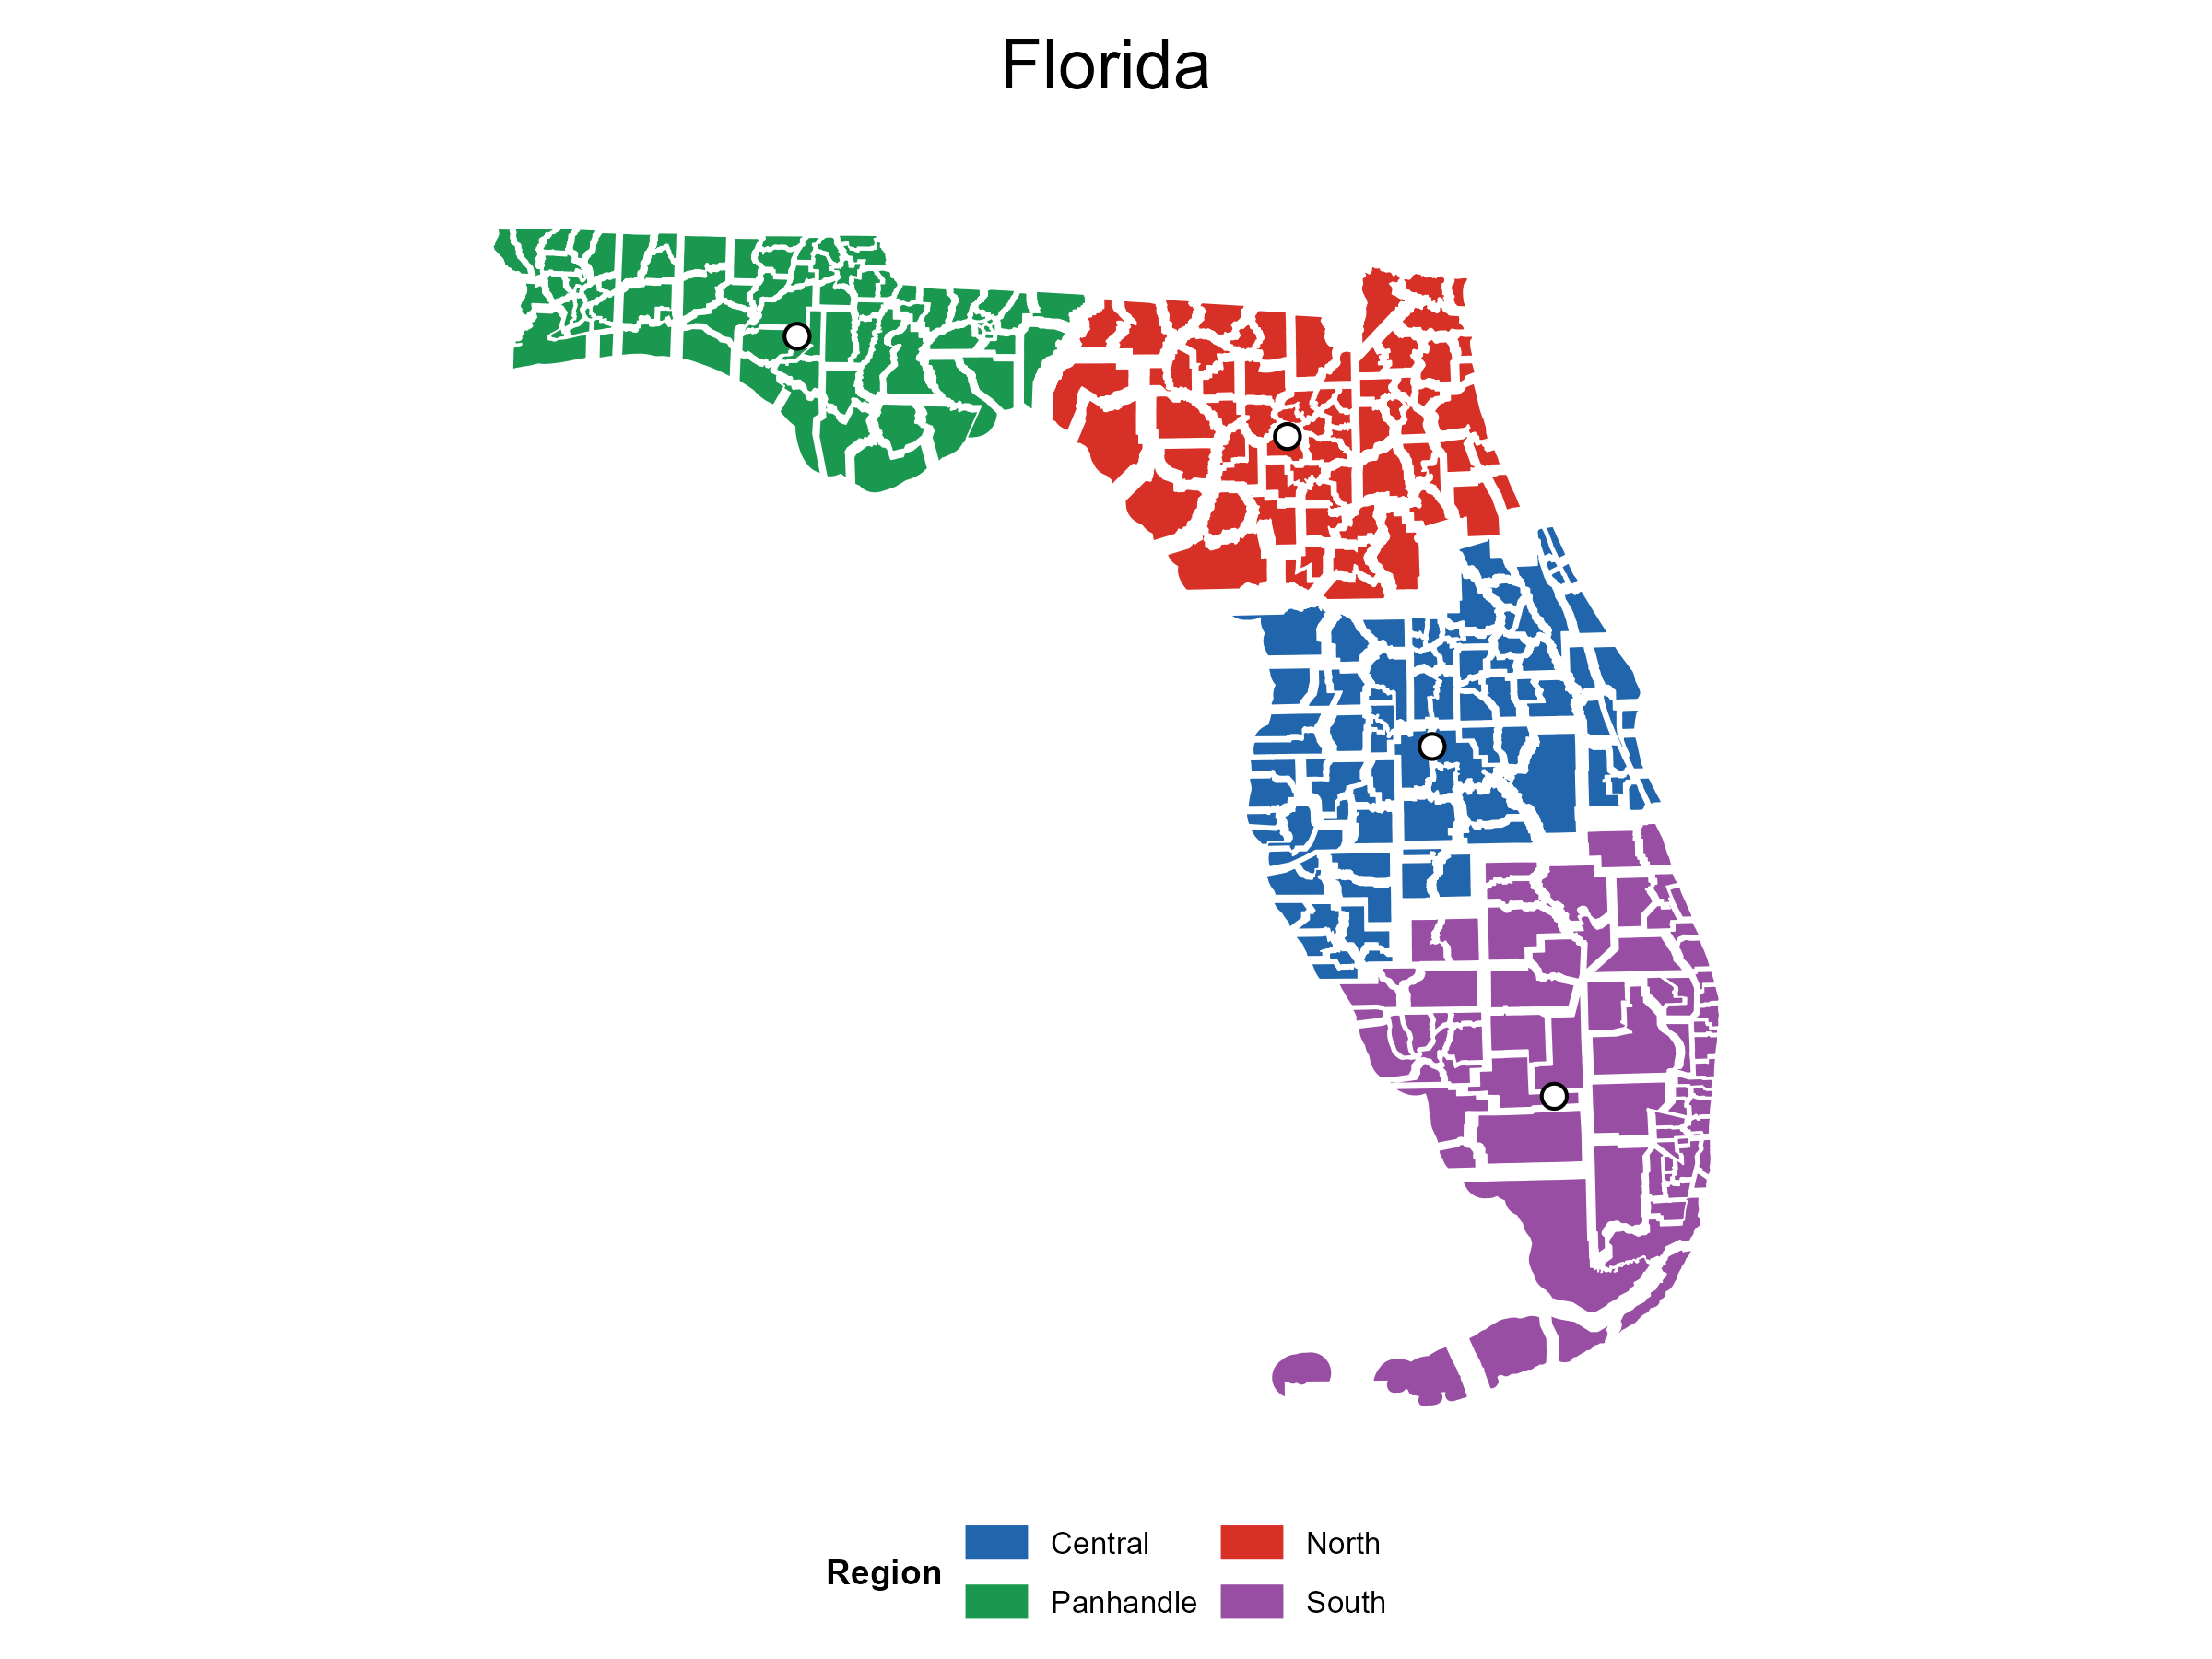
\includegraphics[width=0.82\textwidth]{fl_dragged_layout.png}
\caption{Formula-derived output plus documented display offsets: Florida county subdivisions. The compact four-region hierarchy produces a lower tightness ratio than the dense municipal states; display offsets are used for figure composition only.}
\label{fig:florida}
\end{figure}

The equal-area partition model (Analytical Result~2) also performed correctly: $\alpha_l$ was computed from the median regional radius and median unit count, both of which reflect Lower Peninsula structure. The Upper Peninsula's large municipalities expand correctly under the regional displacement term; their local scaling $s_i$ is small relative to $d_{\max,r}$ for the Upper Peninsula region, so they are not over-expanded locally. This is the expected behavior of Proposition~2 applied to a low-density region.

\subsection{Canada: Non-US Stress Case}
\label{sec:canada}

To evaluate the framework outside the US administrative context, the method was applied to Canadian census subdivision (CSD) boundaries from Statistics Canada 2021. The provinces-only Canadian dataset ($n = 5{,}054$ CSDs, 5 regions: Atlantic, Quebec, Ontario, Prairies, and Pacific) occupies a qualitatively different regime on the hierarchical tightness spectrum, with $\widetilde{R}_{\text{local}}/\bar{w} = 111.23$ --- an order of magnitude larger than any US state in Table~\ref{tab:crossstate}. This reflects the vast geographic extent of Canadian provinces relative to municipal unit size.

Applying the geometry-derived formulas with recommended defaults ($\gamma_r = 3.0$, $\gamma_l = 1.136$) yields $\alpha_r = 22{,}165$\,m and $\alpha_l = 76{,}146$\,m. The provinces-only layout produces a substantially more legible result than layouts that include northern territories, whose vast polygons dominate the visual extent. The structural heterogeneity between dense southern CSDs and sparse northern units illustrates the ``large-unit vs.\ dense-municipal'' contrast identified in the tightness ratio discussion (Section~\ref{sec:ratio}), here occurring \emph{within} a single national dataset rather than across states.

The Canadian case shows that the formula-derived parameters provide a workable starting layout even in an extreme tightness-ratio regime, though the visual dominance of very large territorial units suggests that practitioners working with such datasets may benefit from treating territories as a separate hierarchy level or applying the three-level extension (Section~\ref{sec:multiscale}).

\begin{figure}[H]
\centering
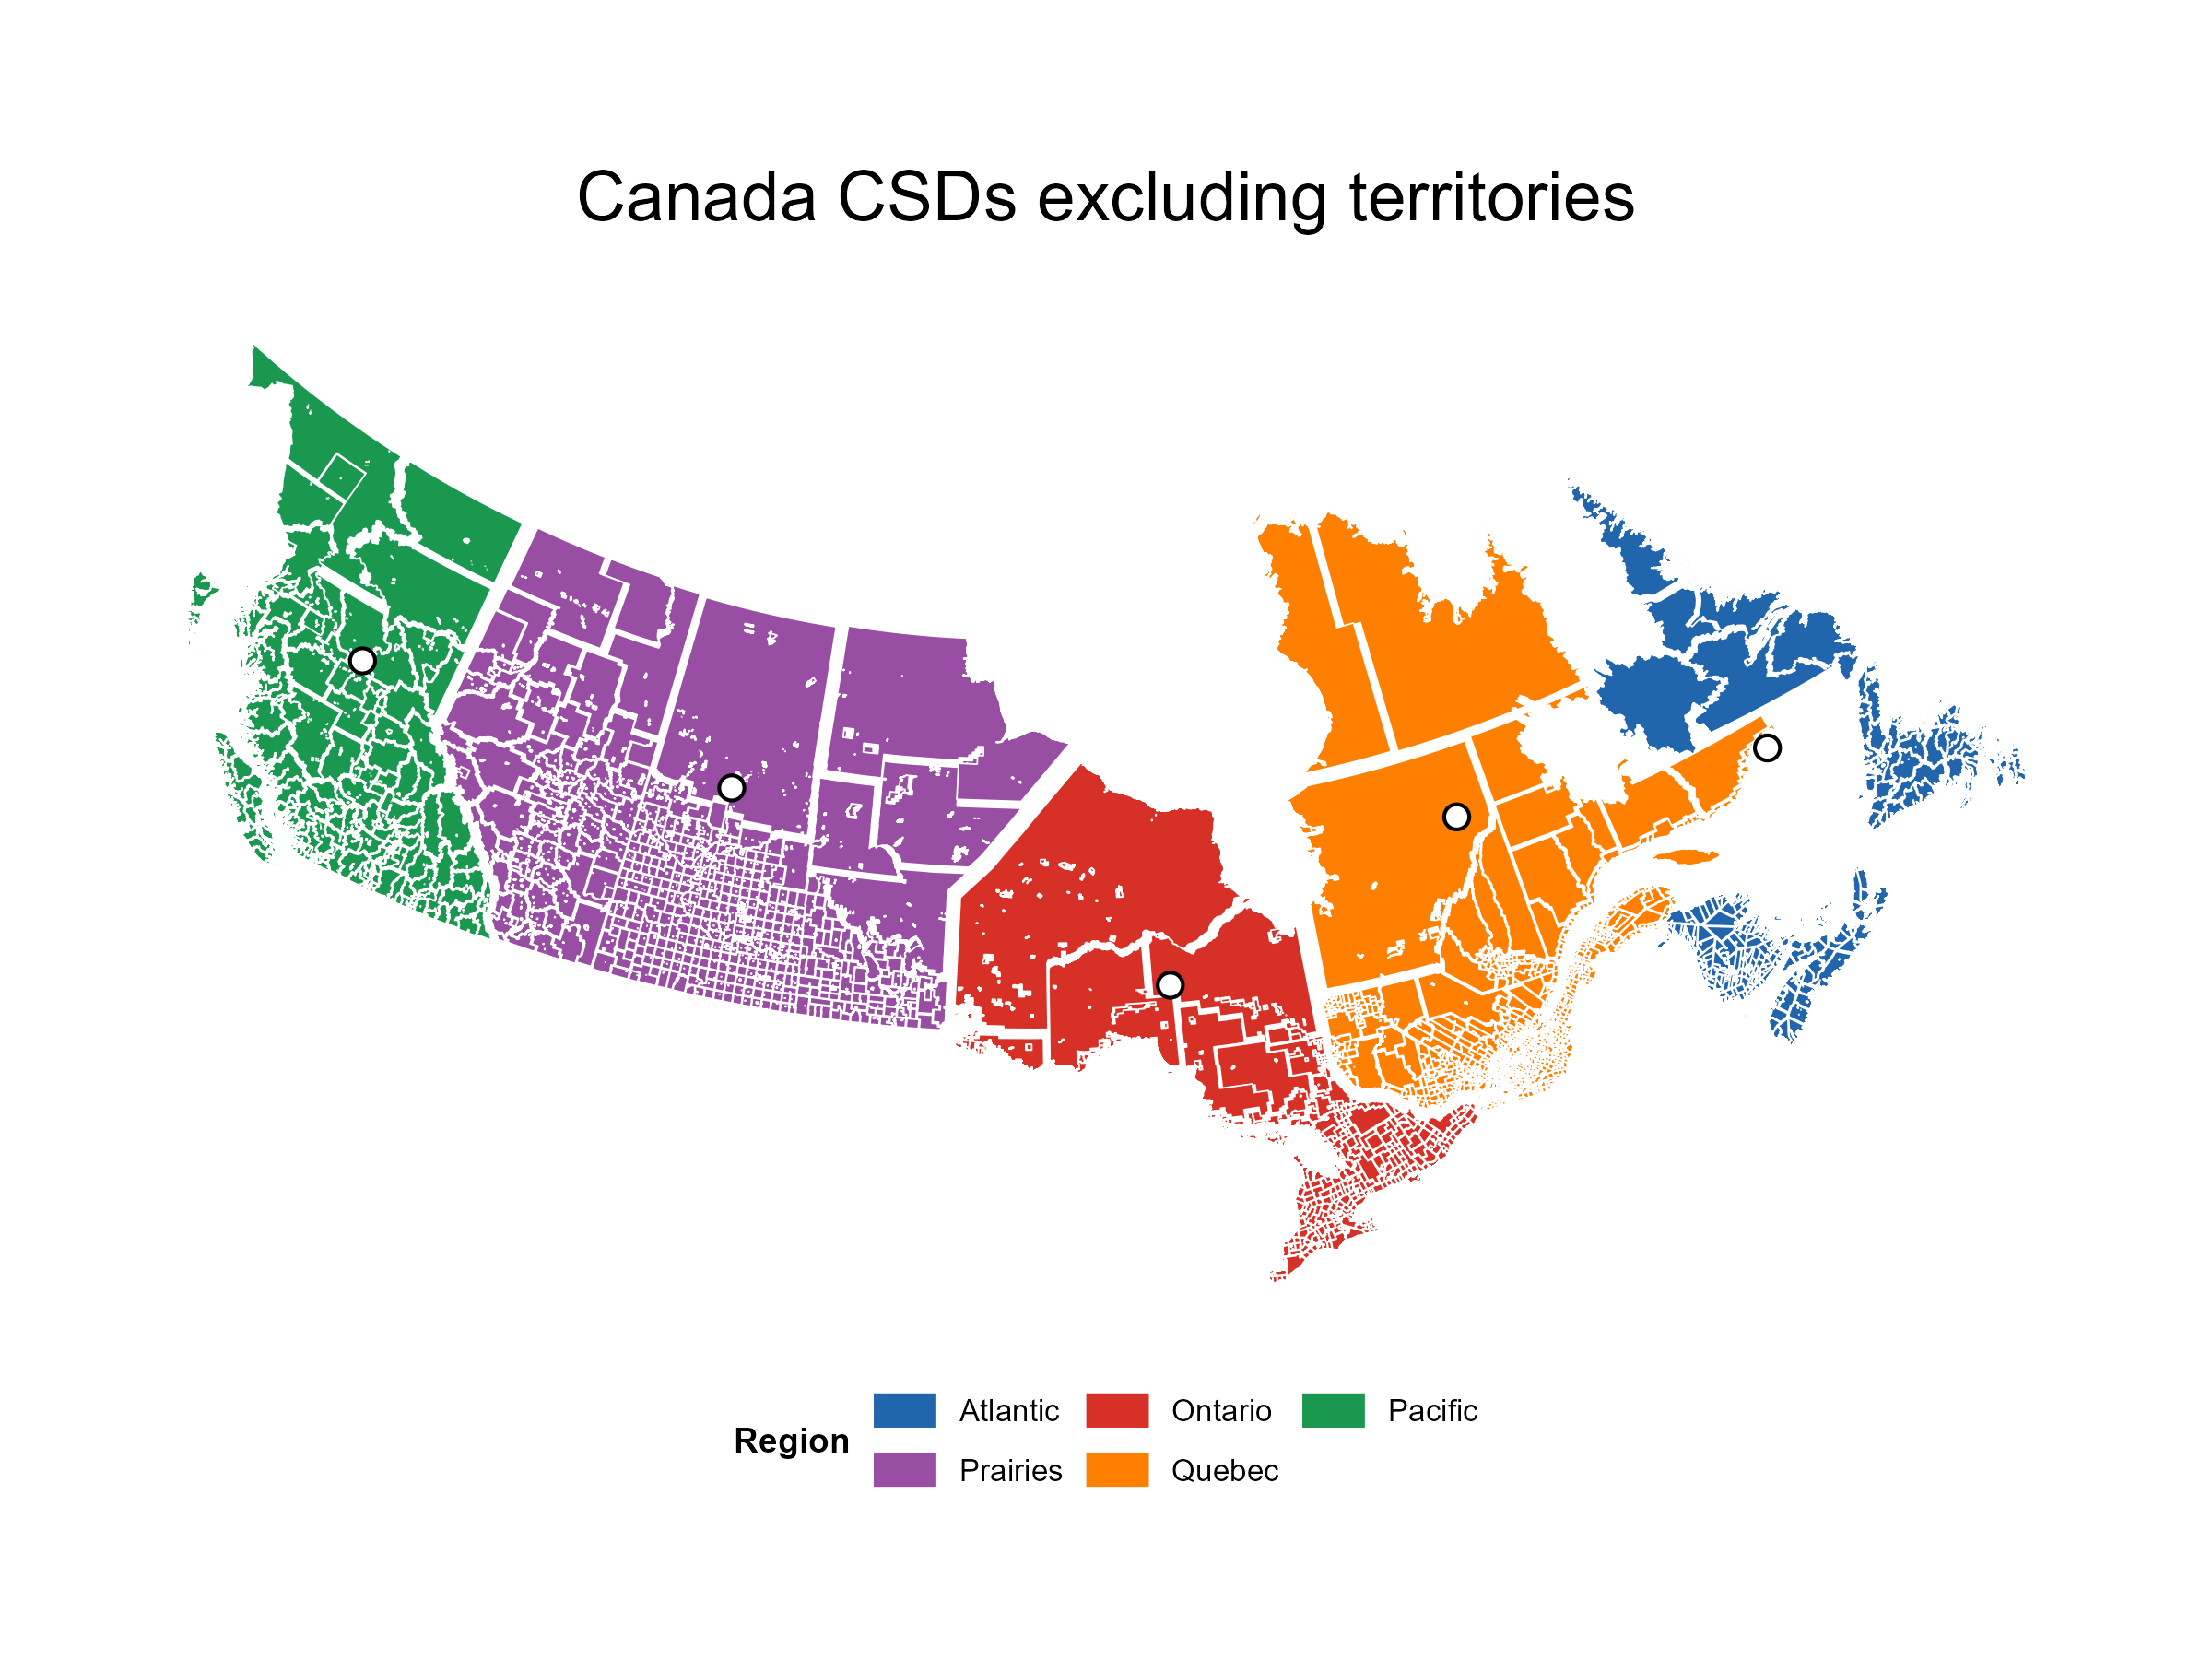
\includegraphics[width=0.82\textwidth]{canada_dragged_layout.png}
\caption{Formula-derived output plus documented display offsets: Canadian census subdivisions, provinces only ($\alpha_r = 22.2$\,km, $\alpha_l = 76.1$\,km, $p = 1.25$, $\gamma_r = 3$, $\gamma_l = 1.136$). Territories are excluded from both this figure and the reported Canada metrics; documented display offsets are applied for figure composition.}
\label{fig:canada_prov}
\end{figure}

\subsection{Germany: Non-US Administrative Regions}

Germany provides a second non-US supplemental example using GADM administrative geometries, grouped by first-level federal states and displayed at a lower administrative level. The result is visually more crowded than the Canadian and U.S.\ state examples because many small units are concentrated in central and western Germany, but the same workflow applies: formula-derived displacement creates the analytical layout, and documented region-level offsets are applied only for final composition.

\begin{figure}[H]
\centering
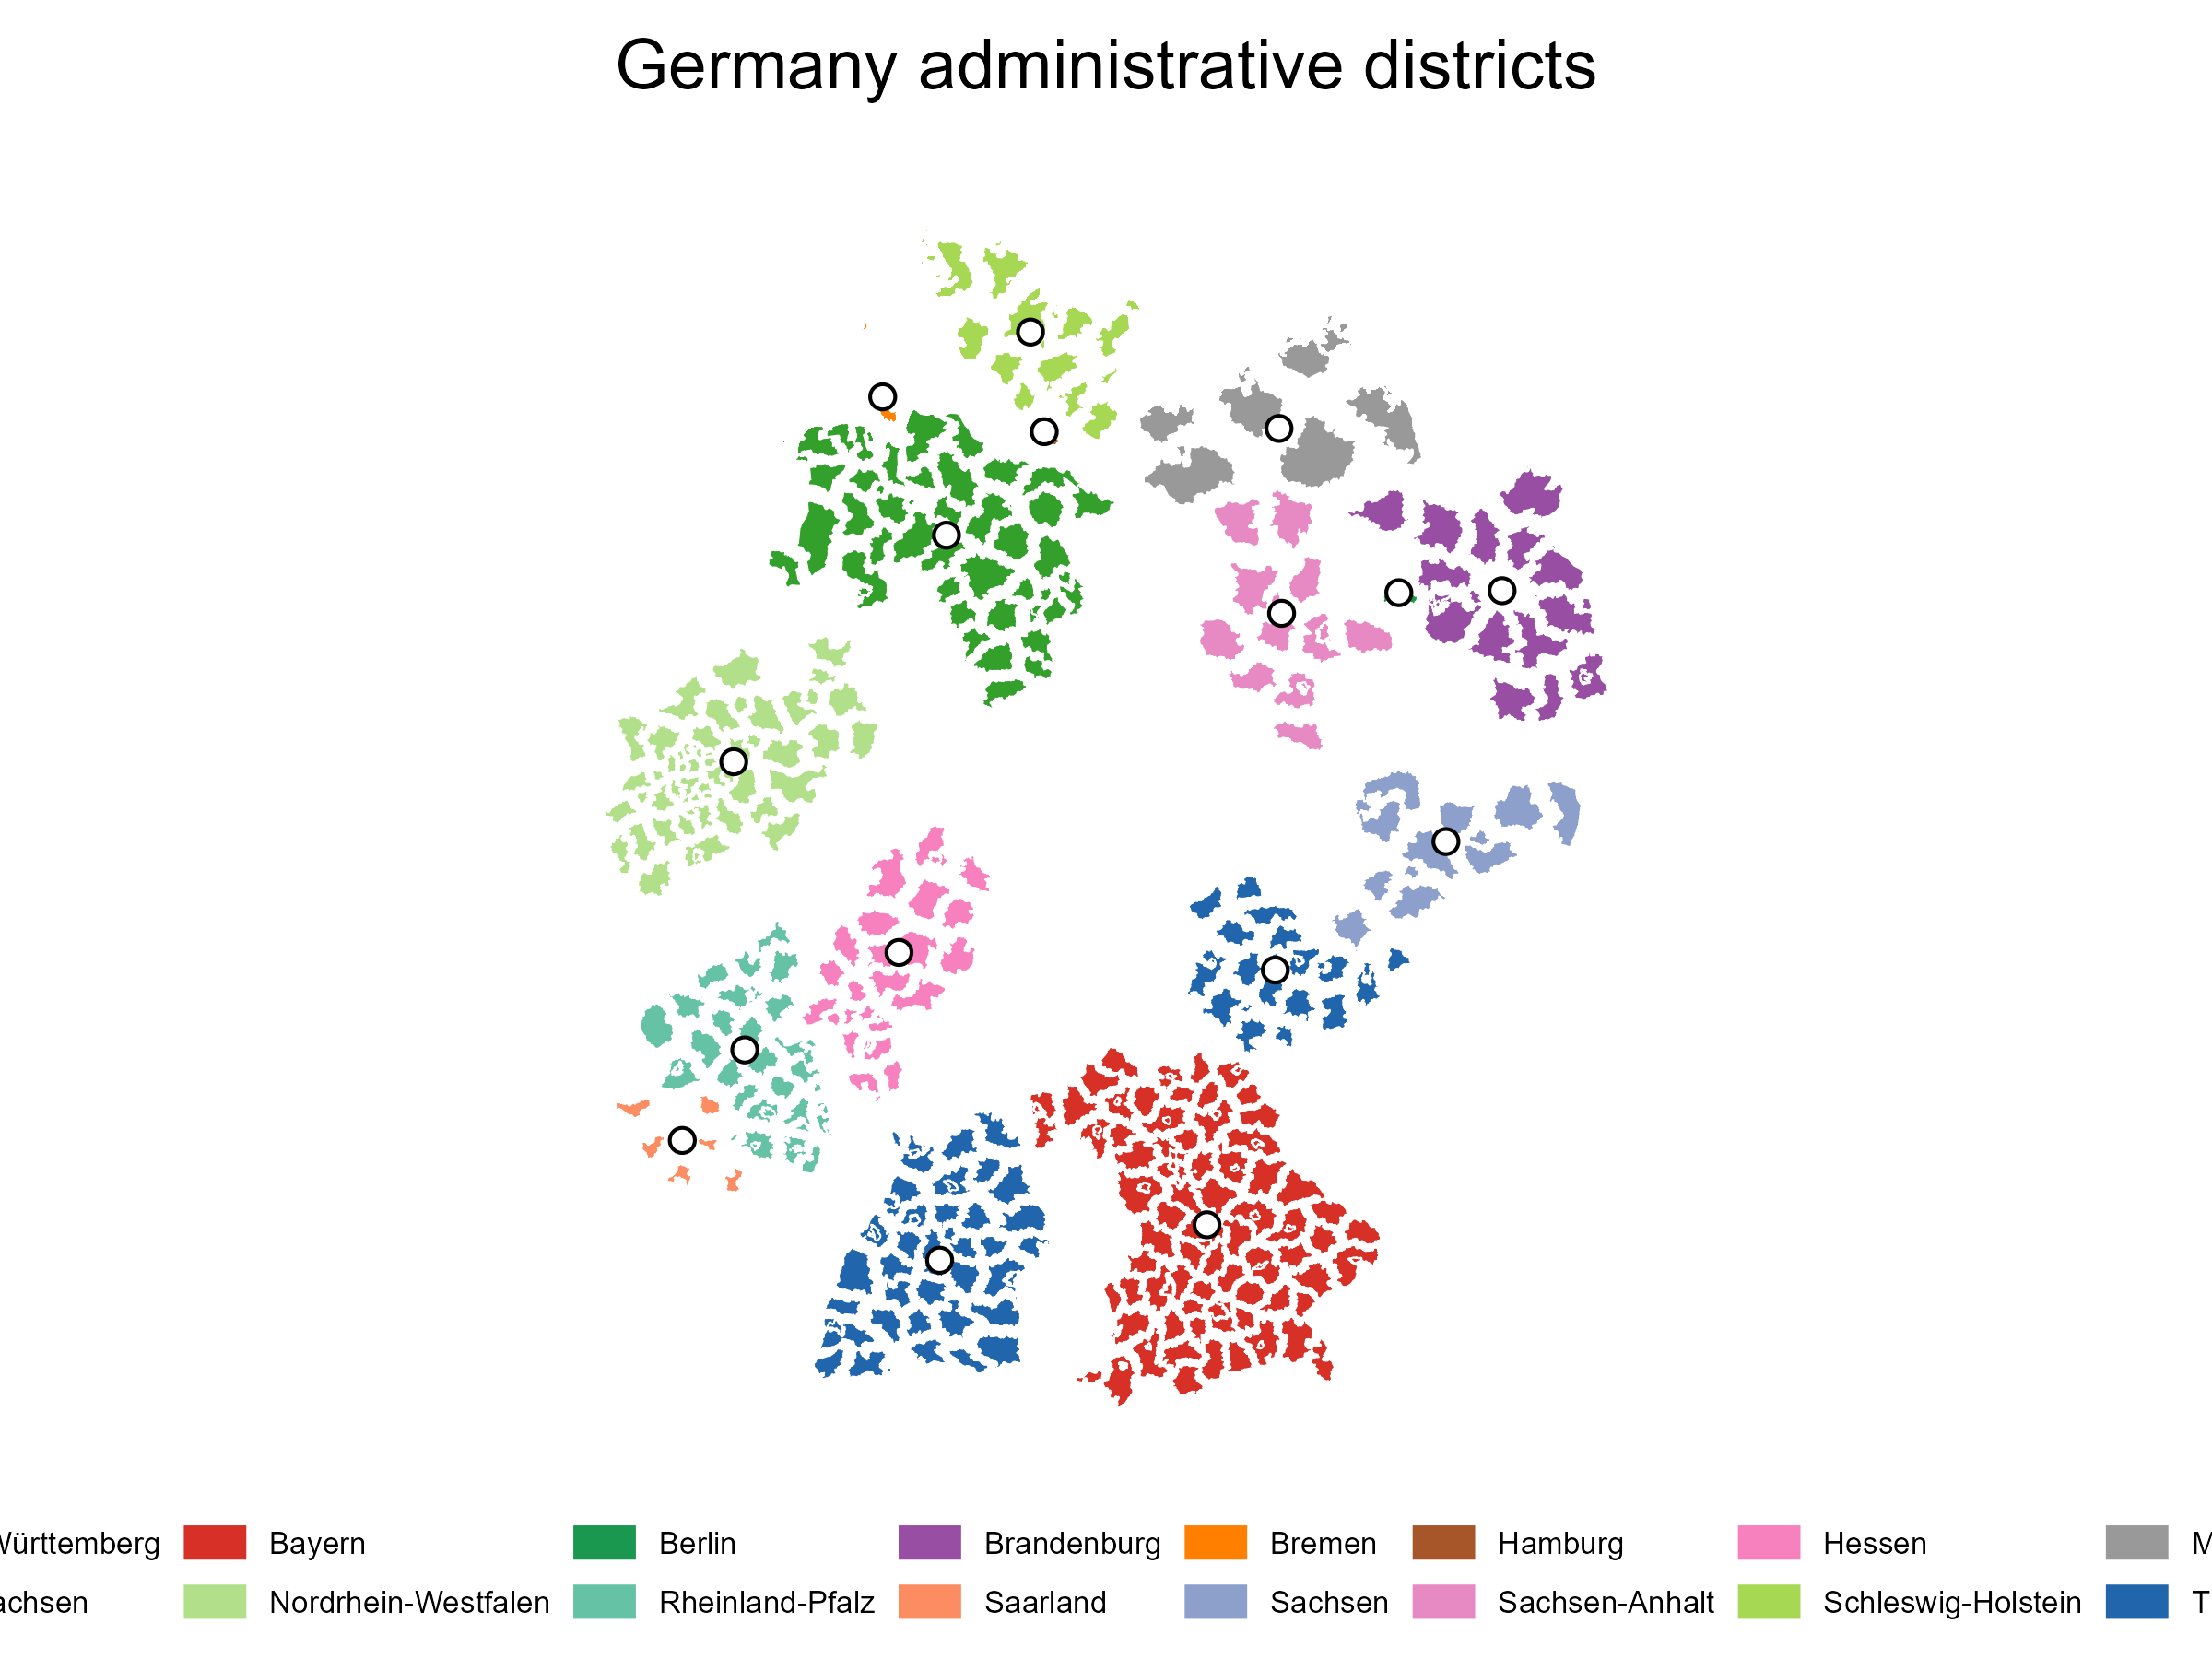
\includegraphics[width=0.82\textwidth]{germany_dragged_layout.png}
\caption{Supplemental stress-test display: Germany administrative regions after formula-derived displacement and documented display offsets. This case is not treated as a full quantitative validation because the administrative density remains high in several neighboring regions and the current manuscript reports it as a visual transfer example.}
\label{fig:germany}
\end{figure}

% ─────────────────────────────────────────────────────────────────────────────
\section{Multi-Scale Extension: National Grouped Layouts}
\label{sec:multiscale}
% ─────────────────────────────────────────────────────────────────────────────

The anchor layout procedure is not a separate algorithm but a direct extension of the hierarchical displacement framework to a higher administrative level. Where the core method operates at two levels (units within regions), the national extension adds a third level (regions within the nation), applying the same centroid-driven displacement logic at each scale.

The core framework operates on two displacement levels: regional separation ($\alpha_r$) and local intra-region expansion ($\alpha_l$). For national maps requiring three-level separation---states within regions, regions within the national extent---the framework extends naturally by introducing \emph{parent-region anchors} that control the gross placement of each region block before the local displacement field is applied.

This yields a three-level displacement hierarchy. Level~1 inherits the exact geometry guarantees of Proposition~1: each administrative unit undergoes rigid-body translation preserving shape, area, and topology. Levels~2 and~3, by contrast, operate at the region-block level and preserve block membership and directional correspondence with the geographic arrangement rather than topological coverage. Thus, the guarantees of Propositions~1--3 apply strictly at Level~1, while higher levels preserve structural grouping rather than topological coverage.

\begin{description}
  \item[Level 1 — Deterministic local explosion.] States within each parent region are displaced using the centroid-driven field (Equation~\eqref{eq:ti}), producing separation within each group. This is the core algorithm unchanged.
  \item[Level 2 — Automatic anchor placement.] Parent region centroids are displaced radially outward from the national centroid $C_{\text{US}}$ to generate initial anchor positions:
  \[
    A_r^{(0)} = C_{\text{US}} + \left(\kappa \cdot \|C_r - C_{\text{US}}\| + \rho + \delta \cdot \log(1 + n_r)\right)\,\hat{u}_r
  \]
  where $\kappa$ is a radial expansion factor, $\rho$ a base padding, $\delta$ a density term, $n_r$ the number of child units in region $r$, and $\hat{u}_r$ the unit vector from the national centroid to $C_r$.
  \item[Level 3 — Collision-aware anchor refinement.] Automatically generated anchors may overlap for densely packed regions. Overlapping anchors are iteratively repelled, while a spring term maintains proximity to the original radial targets:
  \begin{equation}
    A_r^{(t+1)} = A_r^{(t)} + \sum_{s \neq r} F_{rs} + \lambda\left(A_r^{(0)} - A_r^{(t)}\right)
    \label{eq:anchor_update}
  \end{equation}
  where $F_{rs}$ is a repulsion force applied when $\|A_r^{(t)} - A_s^{(t)}\| < R_r + R_s + \rho_{\text{pair}}$, $R_r$ is the block radius of region $r$, and $\lambda$ is the spring coefficient. $F_{rs} = \eta \cdot \frac{(R_r + R_s + \rho_{\text{pair}} - \|A_r - A_s\|)}{2}\,\hat{u}_{rs}$, where $\rho_{\text{pair}}$ is pairwise padding.
\end{description}

\subsection{Block Radius Estimation}

The block radius $R_r$ approximates the spatial extent of region $r$ for collision detection. It is estimated as the 85th percentile of pairwise distances between child-unit centroids and their region centroid:
\[
  R_r = Q_{0.85}\left\{\|C_i - C_r\| : i \in r\right\}
\]
The 85th percentile is preferred over the maximum because the maximum is sensitive to individual outlier units (e.g., Alaska in Region 10 of the HHS classification) and produces over-conservative block radii that push anchors unnecessarily far apart.

\subsection{Spring-Repulsion Balance}

The relative magnitudes of $\lambda$ (spring return) and $\eta$ (dimensionless push fraction) determine the character of the refined layout. Larger $\lambda$ values keep anchors closer to their initial radial positions, while larger $\eta$ values resolve overlaps more aggressively but may reduce geographic correspondence. The present manuscript treats this as an application-level refinement rather than a proved convergence result. Empirically, $\lambda = \eta = 0.18$ with 60 iterations produces compact, radially coherent layouts across the 10-region HHS configuration.

\subsection{Algorithm 2: Anchor Layout Procedure}

\begin{algorithm}[H]
\DontPrintSemicolon
\caption{$\texttt{anchor\_layout}(\mathcal{R}, \kappa, \rho, \delta, \lambda, \eta, T)$. Generates and refines parent-region anchors for the three-level multi-scale layout.}
\KwIn{Regions $\mathcal{R} = \{r\}$; centroids $C_r$; national centroid $C_{\text{US}}$; child counts $n_r$;
      expansion $\kappa$; padding $\rho$; density factor $\delta$; spring $\lambda$; step $\eta$; iterations $T$}
\KwOut{Refined anchor positions $\{A_r\}$; block radii $\{R_r\}$}
\BlankLine
\tcp{Level 2 — Generate initial radial anchors}
\For{each region $r \in \mathcal{R}$}{
  $\hat{u}_r \gets (C_r - C_{\text{US}}) / \|C_r - C_{\text{US}}\|$\;
  $\rho_r \gets \kappa\,\|C_r - C_{\text{US}}\| + \rho + \delta\log(1 + n_r)$\;
  $A_r^{(0)} \gets C_{\text{US}} + \rho_r\,\hat{u}_r$\;
}
\BlankLine
\tcp{Level 3a — Estimate block radii (85th percentile spread)}
\For{each region $r \in \mathcal{R}$}{
  $R_r \gets Q_{0.85}\!\left\{\|C_i - C_r\| : i \in r\right\}$\;
}
\BlankLine
\tcp{Level 3b — Iterative collision resolution with spring return}
\For{$t = 1$ \KwTo $T$}{
  $\Delta_r \gets \mathbf{0}$ for all $r$\;
  \For{each pair $(r, s)$ with $r < s$}{
    $d_{rs} \gets \|A_r^{(t)} - A_s^{(t)}\|$\;
    \If{$d_{rs} < R_r + R_s + \rho_{\text{pair}}$}{
      $\text{overlap} \gets R_r + R_s + \rho_{\text{pair}} - d_{rs}$\;
      Set $\hat{u}_{rs}$ to the unit vector from $A_r^{(t)}$ to $A_s^{(t)}$; if $d_{rs}=0$, use a deterministic radial fallback direction\;
      $F \gets \eta \cdot \tfrac{\text{overlap}}{2} \cdot \hat{u}_{rs}$\;
      $\Delta_r \gets \Delta_r - F$;\quad $\Delta_s \gets \Delta_s + F$\;
    }
  }
  $A_r^{(t+1)} \gets A_r^{(t)} + \Delta_r + \lambda\!\left(A_r^{(0)} - A_r^{(t)}\right)$ for all $r$\;
}
\Return{$\{A_r^{(T)}\}$, $\{R_r\}$}\;
\end{algorithm}

\vspace{4pt}
\noindent\textbf{Complexity.} The collision loop is $O(|\mathcal{R}|^2 \cdot T)$ in the number of regions and iterations. Since $|\mathcal{R}|$ is typically small ($\leq 20$ for national administrative groupings), the anchor refinement step adds negligible overhead relative to the $O(n)$ unit displacement computation.

\subsection{Application: HHS National Layout}

The three-level framework was applied to the 50 US states plus territories assigned to the 10 HHS regions. States were projected to Albers Equal Area (EPSG:5070) for metric consistency. The Level-1 displacement ($\alpha_l = 120{,}000$\,m, $p = 1.25$) is a demonstration parameter selected for national display scale rather than a geometry-derived validation parameter. Level-2 and Level-3 processing place and refine the 10 HHS region anchors. Non-contiguous territories (HI, PR, AK, VI, GU, MP, AS) are repositioned to inset-style locations through rigid translation, maintaining group membership without disrupting the continental layout.

The final HHS figure combines the grouped-layout engine with documented display offsets selected from the drag helper. Numeric region labels are used instead of a full legend inside the figure to keep the map readable at manuscript size. The labels correspond exactly to HHS Regions 1--10.

\begin{figure}[H]
\centering
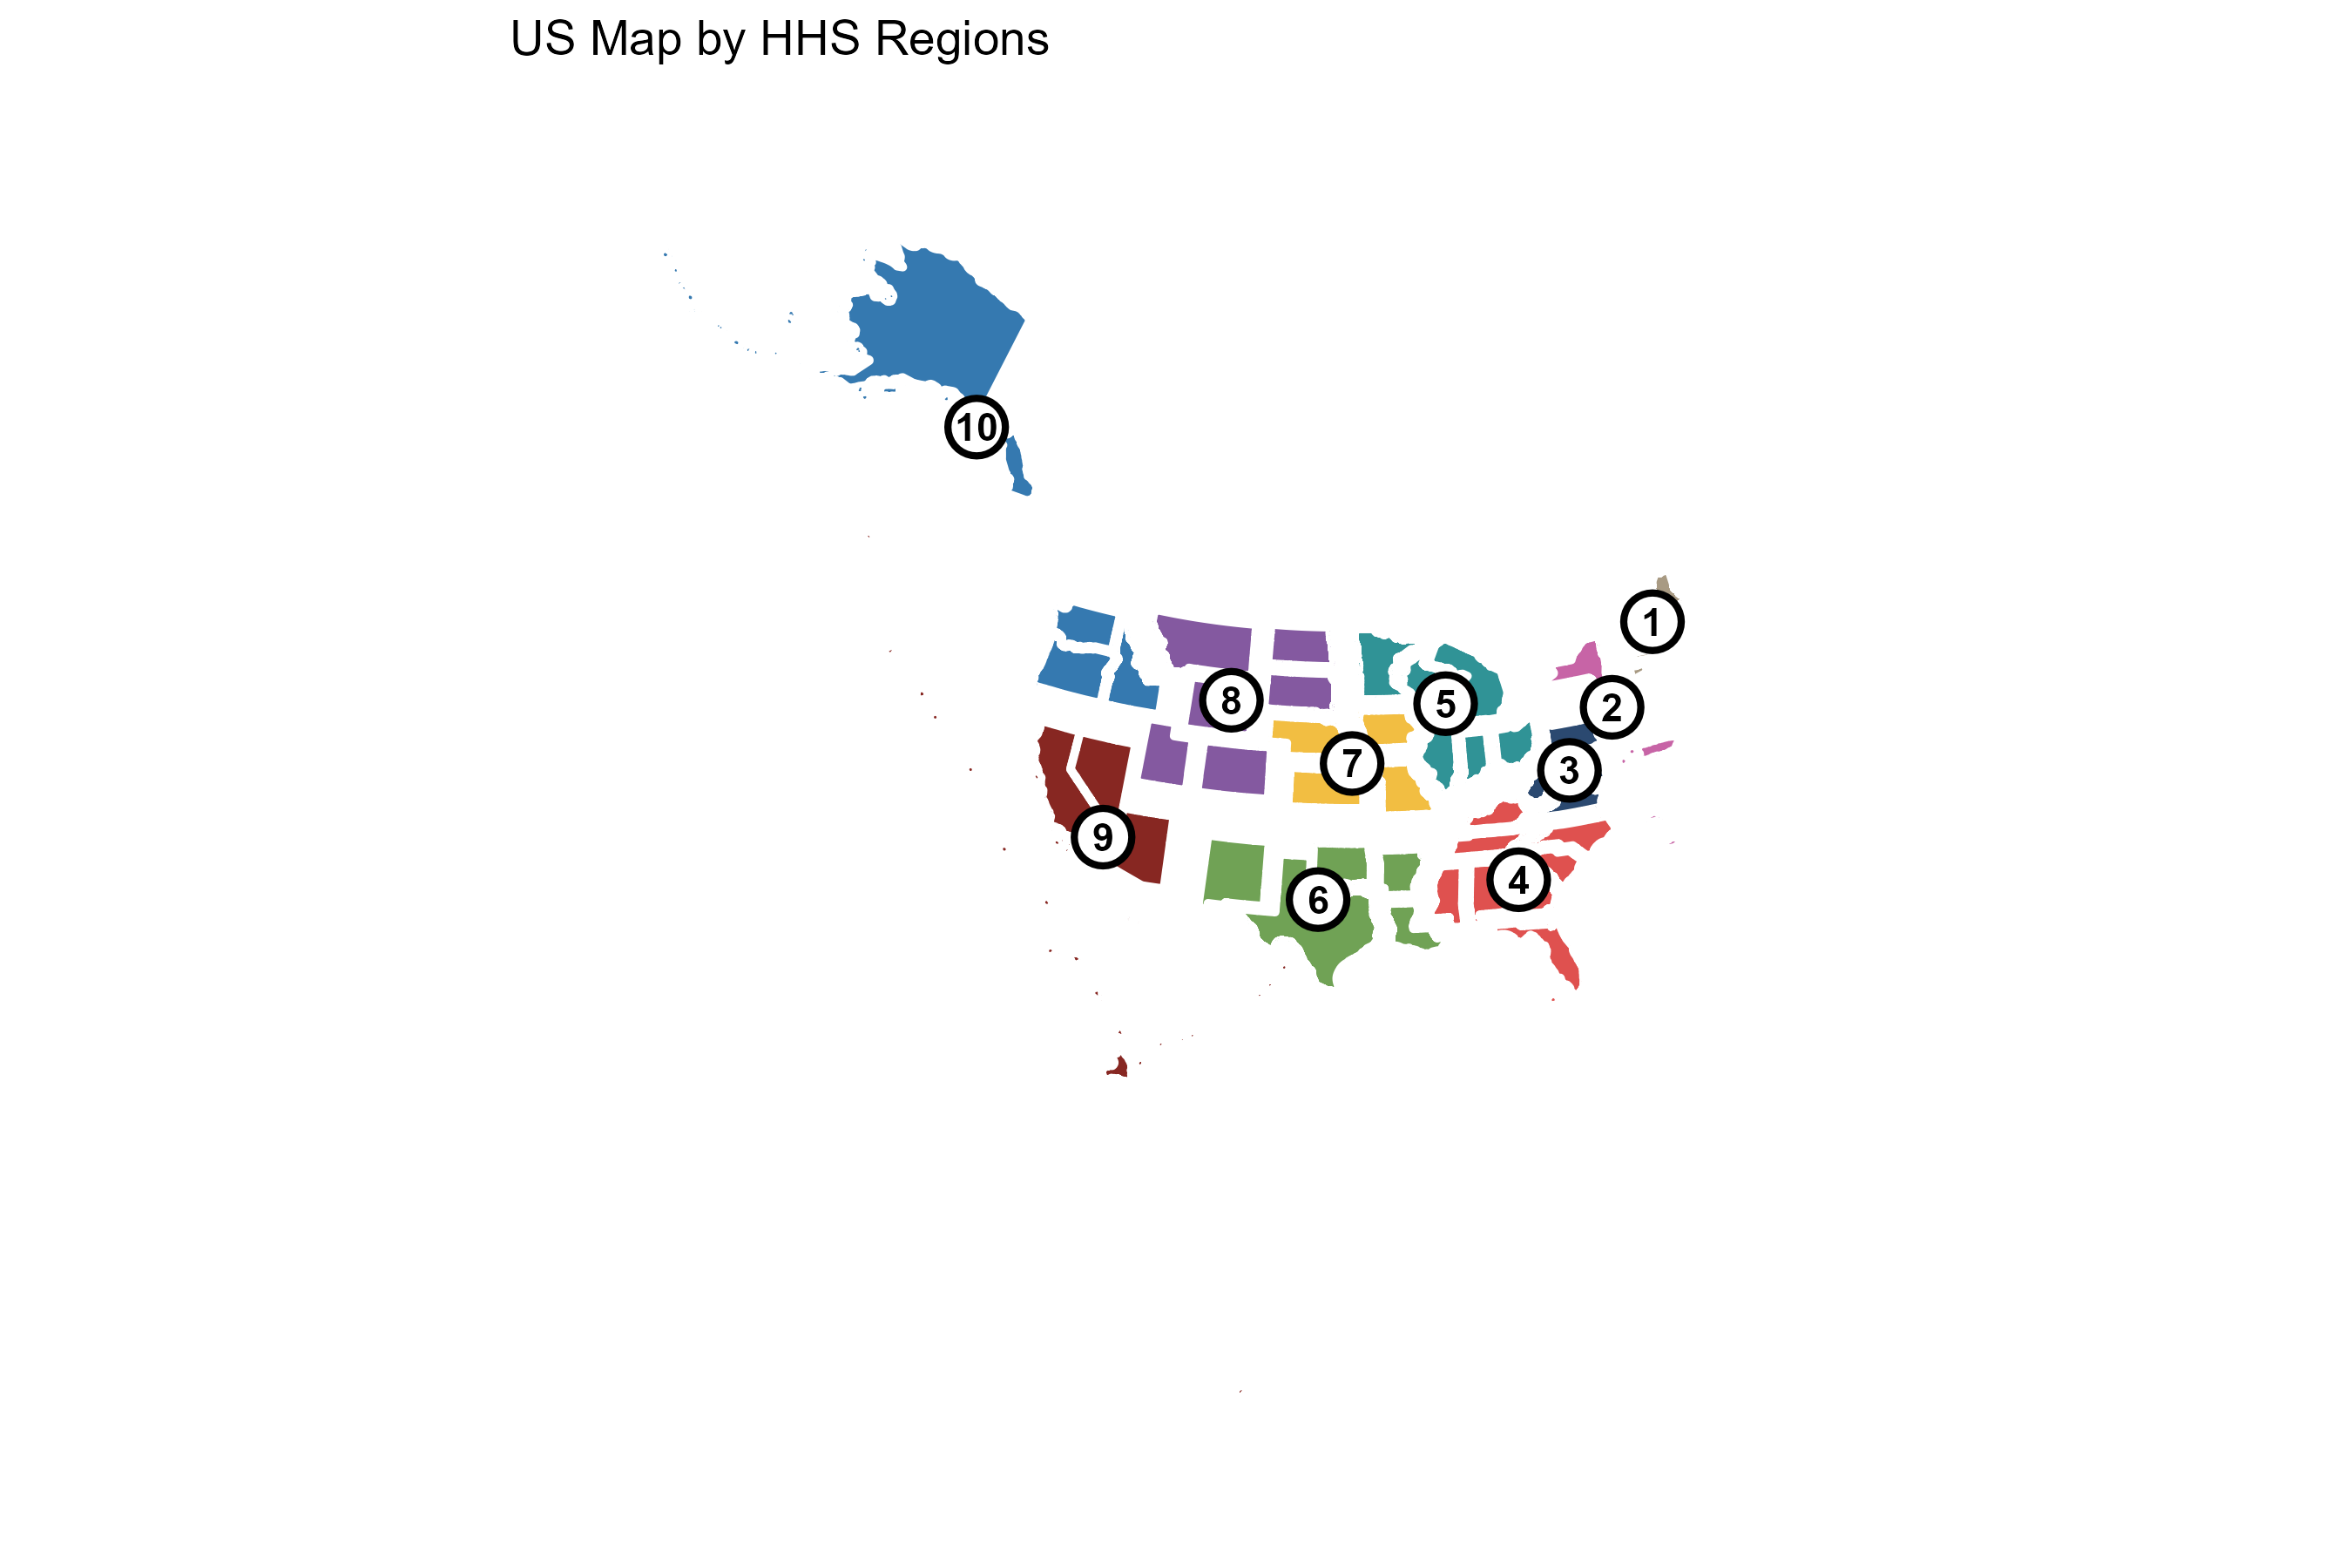
\includegraphics[width=0.82\textwidth]{hhs_dragged_layout.png}
\caption{Formula-derived grouped output plus documented display offsets: HHS national layout with 10 numbered regions. Region numbers match the official HHS region numbering; the offsets are stored in \texttt{paper/outputs/tables/hhs\_drag\_offsets.csv}. This is a multi-level demonstration rather than a quantitative validation of two-level parameter transfer.}
\label{fig:hhs_auto}
\end{figure}

\begin{figure}[H]
\centering
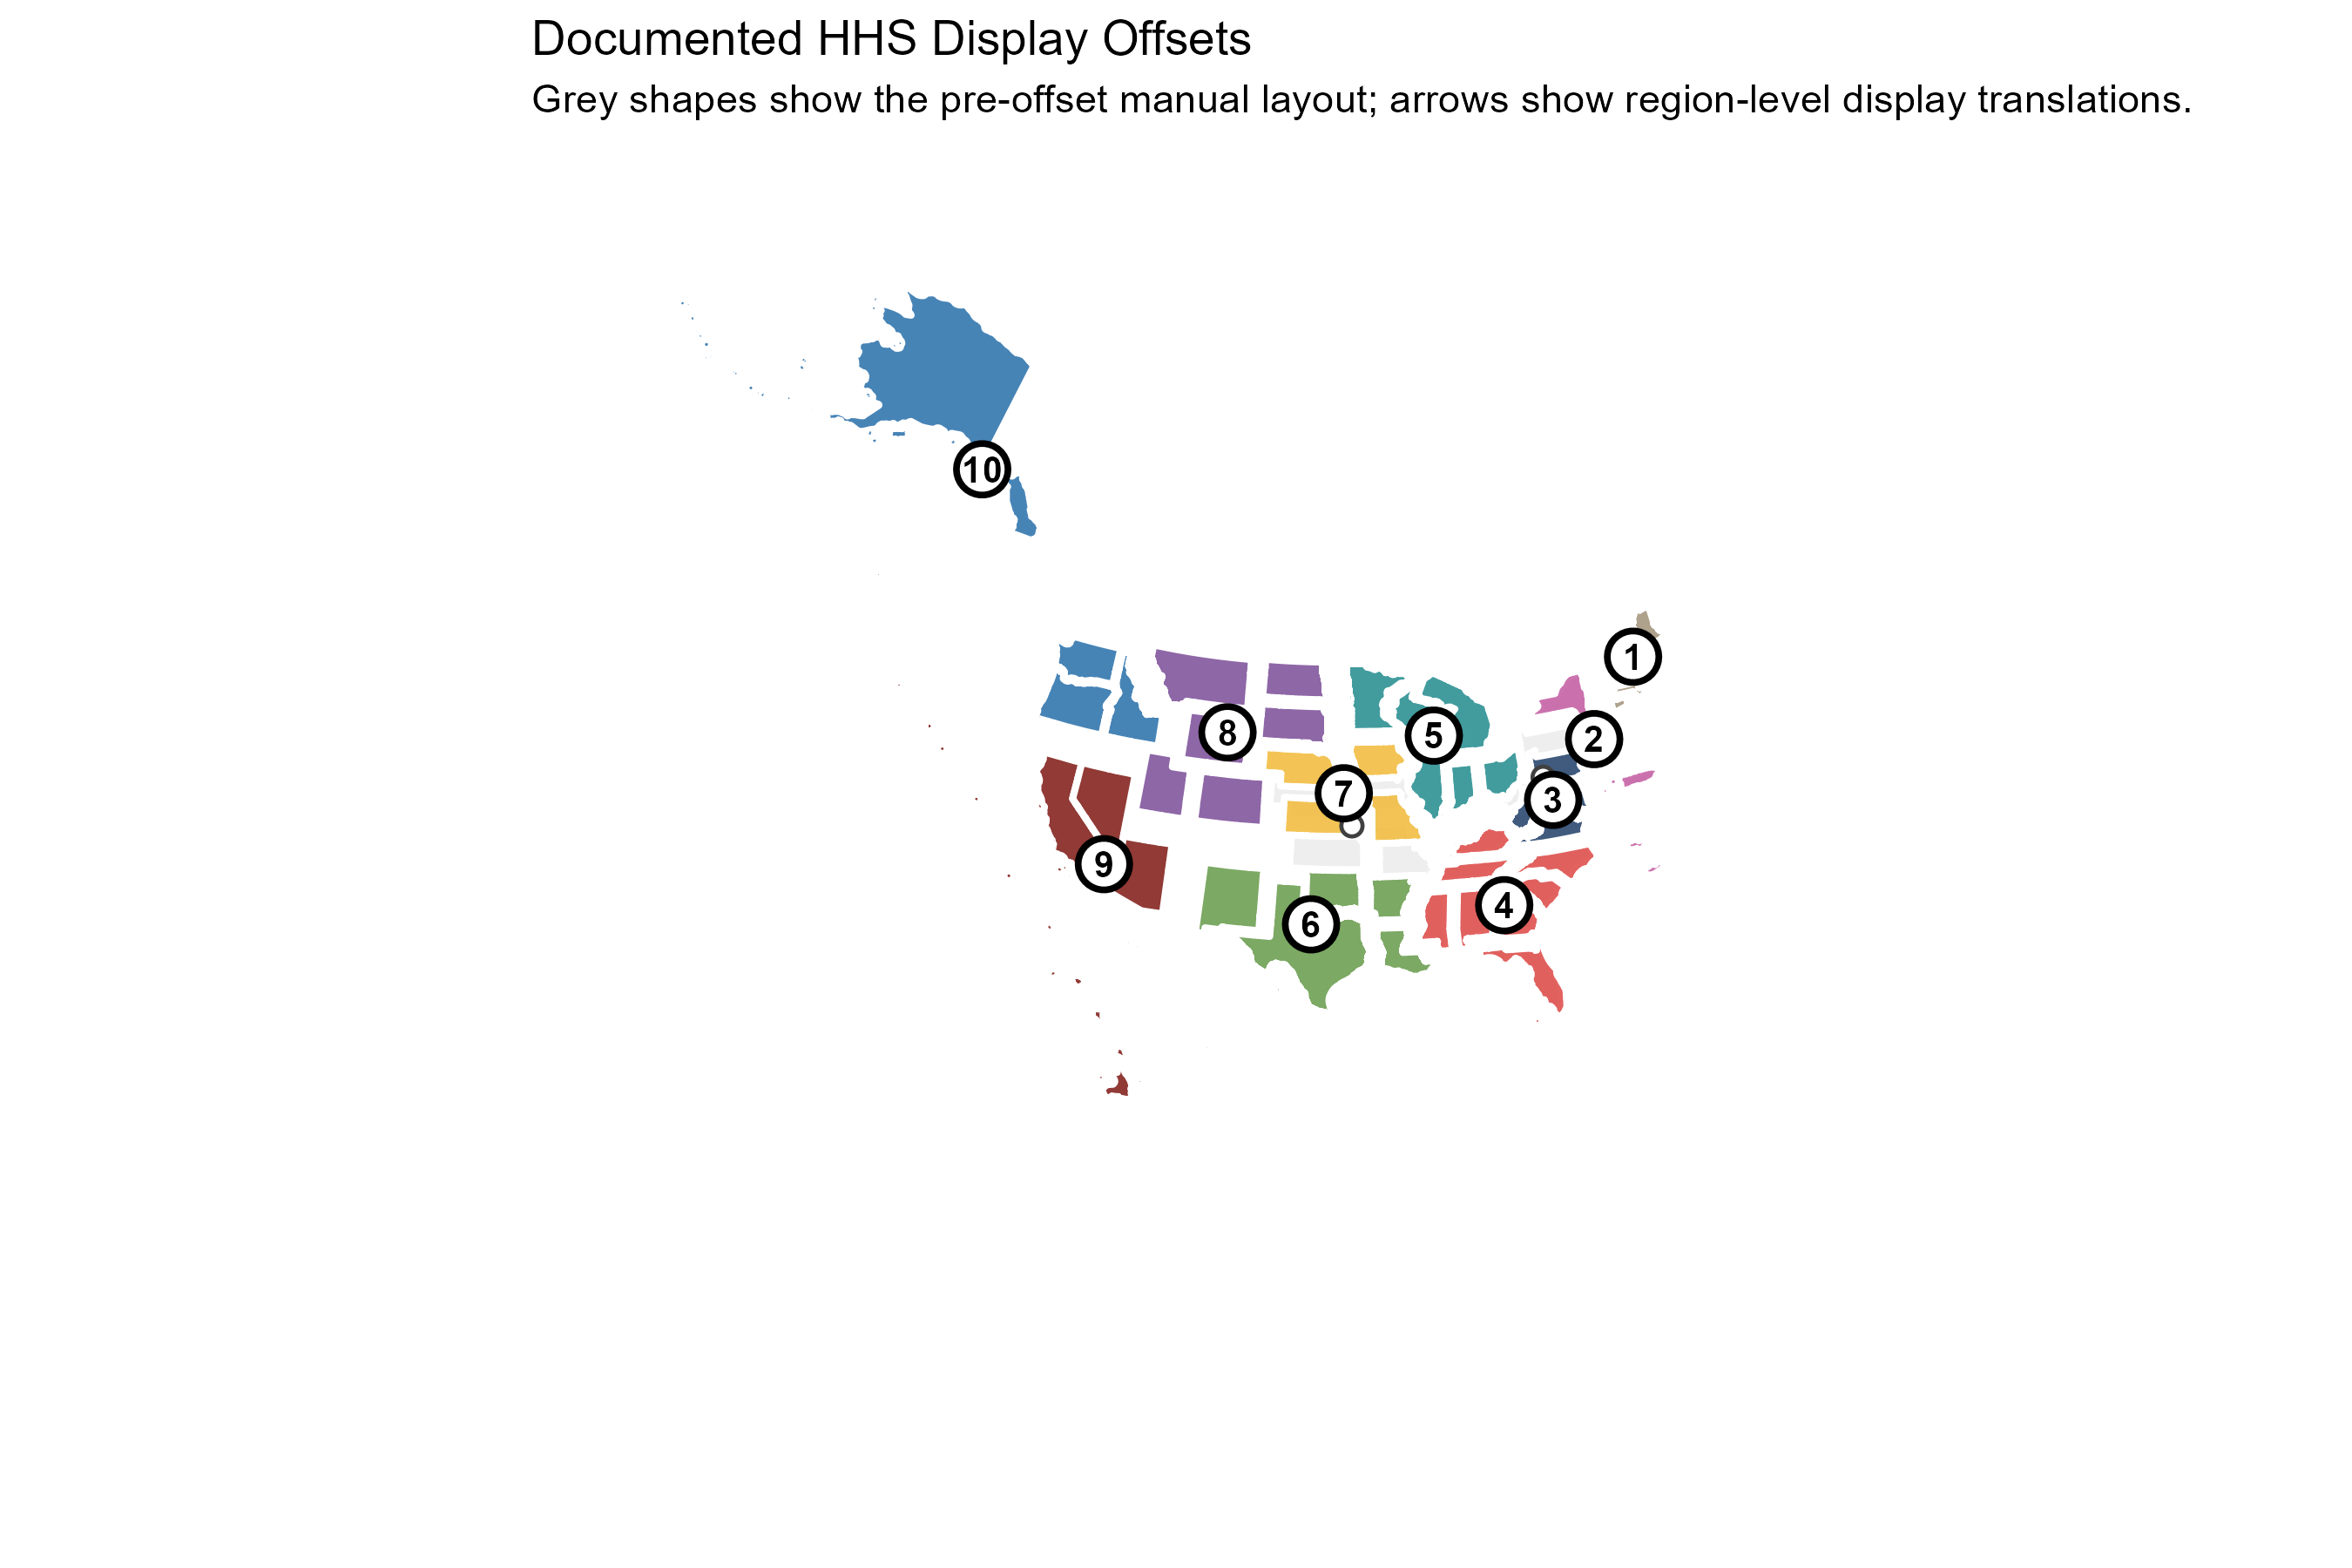
\includegraphics[width=0.82\textwidth]{hhs_display_offsets.png}
\caption{Diagnostic comparison: documented HHS display-offset step. Grey shapes show the pre-offset grouped layout, coloured shapes show the final display layout, and arrows show the region-level translations selected with the drag helper.}
\label{fig:hhs_offsets}
\end{figure}

\begin{table}[H]
\centering
\caption{HHS numeric labels and region membership used in Figure~\ref{fig:hhs_auto}.}
\label{tab:hhs_labels}
\begin{adjustbox}{max width=\textwidth}
\begin{tabular}{lp{0.78\textwidth}}
\toprule
\textbf{Label} & \textbf{HHS region membership} \\
\midrule
1 & Region 1 -- Boston: Connecticut, Maine, Massachusetts, New Hampshire, Rhode Island, and Vermont. \\
2 & Region 2 -- New York: New Jersey, New York, Puerto Rico, and the Virgin Islands. \\
3 & Region 3 -- Philadelphia: Delaware, District of Columbia, Maryland, Pennsylvania, Virginia, and West Virginia. \\
4 & Region 4 -- Atlanta: Alabama, Florida, Georgia, Kentucky, Mississippi, North Carolina, South Carolina, and Tennessee. \\
5 & Region 5 -- Chicago: Illinois, Indiana, Michigan, Minnesota, Ohio, and Wisconsin. \\
6 & Region 6 -- Dallas: Arkansas, Louisiana, New Mexico, Oklahoma, and Texas. \\
7 & Region 7 -- Kansas City: Iowa, Kansas, Missouri, and Nebraska. \\
8 & Region 8 -- Denver: Colorado, Montana, North Dakota, South Dakota, Utah, and Wyoming. \\
9 & Region 9 -- San Francisco: Arizona, California, Hawaii, Nevada, American Samoa, Commonwealth of the Northern Mariana Islands, Federated States of Micronesia, Guam, Marshall Islands, and Republic of Palau. \\
10 & Region 10 -- Seattle: Alaska, Idaho, Oregon, and Washington. \\
\bottomrule
\end{tabular}
\end{adjustbox}
\end{table}

The result demonstrates that the framework's vector-field structure can be extended to a third administrative scale without modifying the Level-1 rigid translation model. It should be interpreted as an application prototype and grouped-layout demonstration, not as a full validation of scale-invariant parameter transfer.

It is worth noting that the collision-aware anchor refinement introduced at the block level in this section --- iterative repulsion with a spring return term operating on a small set of anchor pairs --- is structurally analogous to a potential unit-level bounded refinement for residual polygon conflicts in the two-level framework. In both cases, the analytical displacement field provides a principled initial layout, and a local solver corrects the small number of remaining spacing violations without discarding the hierarchical structure. The block-level version resolves anchor overlaps among $|R|$ regions; the unit-level analogue would resolve boundary contacts among density-driven conflict pairs identified in Section~\ref{sec:evaluation}. This suggests a unified refinement architecture applicable at any level of the displacement hierarchy.

% ─────────────────────────────────────────────────────────────────────────────
\section{Conclusion}
% ─────────────────────────────────────────────────────────────────────────────

This paper presented a hierarchical vector-based framework for multi-scale exploded-view cartography of dense administrative maps. The method defines displacement as a deterministic field derived from hierarchical centroid relationships and applies this field through rigid polygon translation, preserving exact geometry while improving spatial legibility.

Two structural properties underpin the method's correctness. Proposition~1 establishes that rigid-body translation preserves all internal polygon geometry exactly --- shape, area, perimeter, and topology. Proposition~2 establishes that the distance-scaled local expansion preserves the radial ordering of units within each region, guaranteeing that the exploded layout expands coherently outward rather than shuffling or crossing units. Together these properties explain both the mathematical correctness and the perceptual stability of the exploded output.

A central contribution beyond the displacement algorithm is a geometry-derived parameter estimation procedure grounded in two geometric idealizations. Analytical Result~1 (radial gap criterion) derives the functional form of $\alpha_r$ from a radial arrangement model, showing that regional displacement scales as $\gamma_r\,\bar{w} / (2\sin(\pi/n_r))$. Analytical Result~2 (equal-area partition) derives the form of $\alpha_l$ from the equivalent-circle diameter of a typical municipal cell, giving $\gamma_l \cdot 2R_{\text{local}}/\sqrt{\bar{n}}$. The functional dependence on geometry is derived analytically from idealized spatial models; the residual dimensionless coefficients $\gamma_r$ and $\gamma_l$ are cartographic legibility coefficients encoding human readability requirements rather than geometric constraints. The local coefficient $\gamma_l = 1.136$ is supported as a practical default by NJ calibration and transfer results in the current cases; the regional coefficient $\gamma_r$ is directionally consistent but requires additional visual validation.

The extended evaluation covering eleven US states plus Canada and Germany shows that the dimensionless ratio $\widetilde{R}_{\text{local}}/\bar{w}$ is a useful diagnostic of administrative tightness. Fine-grained township states including NJ (15.83), PA (17.26), IL (16.44), ND (18.76), NC (15.27), OH (12.92), and MI (17.81) occupy a higher ratio band than larger-unit cases such as KY (8.46), VA (10.07), TX (8.56), and FL (7.57), while Canadian provinces occupy a qualitatively different regime at 111.23. Michigan's result is particularly useful: despite a geographic discontinuity between its Upper and Lower Peninsulas and a bimodal municipal size distribution, the median-based $\bar{w}$ remains well behaved.

Future work will address independent visual validation of $\alpha_r$ and $\gamma_l$, comparative baselines against other displacement strategies, and user-study evaluation of layout legibility for specific cartographic tasks. The three-level multi-scale extension introduced in Section~\ref{sec:multiscale} opens a further research direction: determining whether the legibility coefficients are scale-invariant across administrative levels, and whether the spring coefficient $\lambda$ in the collision-aware refinement can itself be derived geometrically from regional density structure. The generalized \texttt{explodemap} package implementation enables the framework to be applied across administrative polygon datasets, supporting both further empirical calibration and practical deployment in cartographic production workflows.

The derived parameter formulas constitute a reusable procedure for exploded-view cartography. Any administrative polygon dataset with a defined two-level hierarchy can generate formula-derived starting parameters directly from its geometric properties --- characteristic polygon diameter, regional radius, median unit count, and number of regions --- without case-specific manual tuning.

\subsection*{Code Availability}

The reference implementation is available as an MIT-licensed \textsf{R} package, a set of reproducible paper scripts, and an interactive Shiny validation application. The outputs and gallery used in this manuscript correspond to package version \texttt{0.2.0} and repository commit \texttt{e937206}; a versioned archive DOI should be minted before journal submission. The core release includes:
\begin{itemize}
  \item \texttt{explode\_sf()}, \texttt{explode\_state()}, and \texttt{explode\_sf\_with\_lookup()} --- generalized entry points applicable to projected polygon datasets with arbitrary grouping columns, lookup tables, or U.S.\ state TIGER/Line inputs.
  \item \texttt{explode\_grouped()} --- three-level national and multi-region grouped layouts with collision-aware anchor refinement (Algorithm~2).
  \item \texttt{apply\_region\_offsets()} --- reproducible application of documented region-level display offsets stored as CSV files.
  \item Installed example scripts in \texttt{inst/examples/} --- reproducible calibration, Canada, HHS, lookup-table, manual-tuning, collision-refinement, and focus-map workflows.
  \item Shiny focus-map examples --- interactive selected-feature inspection with \texttt{focusmapOutput()} and \texttt{renderFocusmap()}.
  \item \texttt{focus\_map()} --- companion htmlwidget for selected-feature viewport focusing, non-blocking information cards, and Shiny integration; its interaction mathematics are developed separately from the exploded-view displacement model.
\end{itemize}
All case studies are reproducible from public U.S.\ Census TIGER/Line, Statistics Canada, and GADM boundary data using the scripts and offset tables in \texttt{paper/scripts} and \texttt{paper/outputs/tables}. No proprietary data or software is required. The package checks can be run with \texttt{R CMD check}, and the manuscript can be rebuilt from \texttt{paper/explodemap\_paper.tex} with \texttt{pdflatex} after regenerating figures from the scripts in \texttt{paper/scripts}.

\subsection*{Interactive Map Gallery}

An accompanying interactive gallery is available at \url{https://prigasg.github.io/explodemap/map-gallery/index.html}. The package repository is available at \url{https://github.com/PrigasG/explodemap}. The gallery corresponds to package version \texttt{0.2.0}; accessed May 26, 2026.

The gallery is intended to make the distinction between analytical outputs and publication-display outputs explicit. It includes New Jersey, Pennsylvania, extended U.S.\ state examples, Canada and Germany, and the national HHS grouped layout. For each case, the page lists the parameters used, whether documented display offsets were applied, and links to the corresponding offset CSV files. The display-offset layouts are used for publication figures and web comparison, but the validation metrics in this paper are computed from the original geography and the formula-derived exploded layouts unless otherwise stated.
The same output taxonomy is defined earlier in Table~\ref{tab:output-types} so that readers encounter it before the case-study figures.

% ─────────────────────────────────────────────────────────────────────────────
\bibliographystyle{plainnat}
\begin{thebibliography}{99}

\bibitem[Steiniger \& Weibel(2007)]{steiniger2007}
Steiniger, S., \& Weibel, R. (2007).
Relations among map objects in cartographic generalization.
\textit{Cartography and Geographic Information Science}, 34(3), 175--197.
\url{https://doi.org/10.1559/152304007781697866}

\bibitem[Bouts et~al.(2015)]{bouts2015}
Bouts, Q.~W., Dwyer, T., \& Dykes, J. (2015).
Visual encoding of dissimilarity data via topology-preserving map deformation.
\textit{IEEE Transactions on Visualization and Computer Graphics}, 21(9), 1037--1050.
\url{https://openaccess.city.ac.uk/id/eprint/15023/}

\bibitem[Ngo et~al.(2019)]{ngo2019}
Ngo, P., Passat, N., Kenmochi, Y., \& Talbot, H. (2019).
Geometric preservation of 2D digital objects under rigid motions.
\textit{Journal of Mathematical Imaging and Vision}, 61(2), 204--223.
\url{https://doi.org/10.1007/s10851-018-0842-9}

\bibitem[van Lieshout(2010)]{vanlieshout2010}
van Lieshout, M.~C. (2010).
Spatial point process theory.
In A.~E. Gelfand, P.~J. Diggle, M.~Fuentes, \& P.~Guttorp (Eds.),
\textit{Handbook of Spatial Statistics} (pp.~263--282). CRC Press.

\bibitem[Ai et~al.(2015)]{ai2015}
Ai, T., Zhang, X., Zhou, Q., \& Yang, M. (2015).
A vector field model to handle the displacement of multiple conflicts in building generalization.
\textit{International Journal of Geographical Information Science}, 29(8), 1310--1331.
\url{https://doi.org/10.1080/13658816.2015.1019886}

\bibitem[Bader(2001)]{bader2001}
Bader, M. (2001).
\textit{Energy minimization methods for feature displacement in map generalization}.
Doctoral dissertation, University of Zurich.

\bibitem[Bundy et~al.(2020)]{bundy2020}
Bundy, G., Jones, C.~B., \& Furse, E. (2020).
Holistic generalization of large-scale cartographic data.
In \textit{GIS and Generalisation}. Taylor \& Francis.

\bibitem[Cecconi(2003)]{cecconi2003}
Cecconi, A. (2003).
\textit{Integration of cartographic generalization and multi-scale databases for enhanced web mapping}.
Doctoral dissertation, ETH Zurich.

\bibitem[Gastner \& Newman(2004)]{gastner2004}
Gastner, M.~T., \& Newman, M.~E.~J. (2004).
Diffusion-based method for producing density-equalizing maps.
\textit{Proceedings of the National Academy of Sciences}, 101(20), 7499--7504.
\url{https://doi.org/10.1073/pnas.0400280101}

\bibitem[Harrie \& Sarjakoski(2002)]{harrie2002}
Harrie, L., \& Sarjakoski, T. (2002).
Simultaneous graphic generalization of vector data sets.
\textit{GeoInformatica}, 6(3), 233--261.

\bibitem[Jenny \& Hurni(2011)]{jenny2011}
Jenny, B., \& Hurni, L. (2011).
Studying cartographic heritage: Analysis and visualization of geometric distortions.
\textit{Computers \& Graphics}, 35(2), 170--178.

\bibitem[Mackaness et~al.(2011)]{mackaness2011}
Mackaness, W.~A., Ruas, A., \& Sarjakoski, L.~T. (2011).
\textit{Generalisation of Geographic Information: Cartographic Modelling and Applications}.
Elsevier.

\bibitem[Nusrat \& Kobourov(2016)]{nusrat2016}
Nusrat, S., \& Kobourov, S. (2016).
The state of the art in cartograms.
\textit{Computer Graphics Forum}, 35(3), 619--642.

\bibitem[Sun(2020)]{sun2020}
Sun, S. (2020).
Applying forces to generate cartograms: a fast and flexible transformation framework.
\textit{Cartography and Geographic Information Science}, 48(1), 1--16.

\bibitem[Wu \& Wang(2021)]{wu2021}
Wu, F., \& Wang, J. (2021).
Cartographic generalization.
In \textit{Advances in Cartography and Geographic Information Science}. Springer.

\bibitem[Yan \& Wang(2019)]{yan2019}
Yan, H., \& Wang, J.~Y. (2019).
\textit{Description Approaches and Automated Generalization Algorithms for Groups of Map Objects}.
Springer.

\bibitem[{U.S.\ Census Bureau}(2024)]{tiger2024}
U.S.\ Census Bureau. (2024).
TIGER/Line Shapefiles: County Subdivisions.
\url{https://www.census.gov/geographies/mapping-files/time-series/geo/tiger-line-file.html}

\end{thebibliography}

\end{document}
